\documentclass[a4paper,11pt,spanish]{book}
%\usepackage[utf8]{inputenc}
\usepackage[utf8x]{inputenc}
\usepackage{url}
\usepackage{makeidx}
\usepackage[procnames]{listings}
\usepackage{color}
\usepackage{graphicx} % graficos
\usepackage{subfig}
\usepackage{tabularx}
%\usepackage{subcaption}
\captionsetup{compatibility=false}
\usepackage[export]{adjustbox}
\usepackage[spanish]{babel}
\usepackage{mathtools}
\usepackage[chapter]{algorithm}
\usepackage{algorithmicx}
\usepackage{algpseudocode}
%\usepackage[options]{natbib}
\usepackage{verbatim, amsmath, amsfonts, amssymb, amsthm} % For code environment and math support

\usepackage{fullpage}


\newcommand*{\FIXME}[1]{{(\textbf{FIXME}) {#1}}}

\iffalse
\let\mylistof\listof
\renewcommand\listof[2]{%
  \mylistof{algorithm}{Lista de Algortimos}%
}
\fi

\iffalse
\title{Transferencia de Estilo en Fotografias utilizando Redes Neuronales Convolucionales}   %note \\[1ex] is a line break in the title

\author{Wolfmann, Ariel Mauricio}             %your name
\college{Facultad de Matemática, Astronomía y Física\\[1ex]
		}  %your college
\university{Universidad Nacional de Córdoba}

%\renewcommand{\submittedtext}{change the default text here if needed}
%\degree{Licenciada en Ciencias de la Computación}     %the degree
\directors{Sanchez, Jorge}
\fi

\makeindex



\begin{document}
\definecolor{keywords}{RGB}{255,0,90}
\definecolor{comments}{RGB}{0,0,113}
\definecolor{red}{RGB}{160,0,0}
\definecolor{green}{RGB}{0,150,0}

\lstset{language=Python,
        basicstyle=\ttfamily\small,
        keywordstyle=\color{keywords},
        commentstyle=\color{comments},
        stringstyle=\color{red},
        showstringspaces=false,
        identifierstyle=\color{green},
        procnamekeys={def,class}}


\begin{titlepage}
  \begin{center}
  \vspace*{1in}
    \begin{Huge}
    \textbf{Trabajo Final}\\
    \textbf{Transferencia de Estilo en Fotografias utilizando Redes Neuronales Convolucionales} \\
    \end{Huge}
  \end{center}
  \begin{center}
    \begin{large}
      \vspace*{1in}
      Autor: Wolfmann, Ariel Mauricio\\
      Director: Sanchez, Jorge\\
    \end{large}
    \vspace*{0.15in}
     Marzo de 2017\\
    \vspace*{0.15in}
    Universidad Nacional de Córdoba\\
    \vspace*{0.15in}
    Facultad de Matemática, Astronomía y Física\\
    \vspace*{0.6in}
  \end{center}
\end{titlepage}

\iffalse
\maketitle                  % create a title page from the preamble info
\include{abstract}          % include the abstract
\include{dedication}        % include a dedication.tex file
\include{acknowlegements}   % include an acknowledgements.tex file

\begin{romanpages}          % start roman page numbering
\tableofcontents            % generate and include a table of contents
\listoffigures              % generate and include a list of figures
\end{romanpages}            % end roman page numbering
\fi

\tableofcontents
%\listoffigures
%\listofalgorithms

\chapter{Introducción}
  \section {Contexto}
    En los últimos años las fotografías están cada vez más, pasando a ser un objeto virtual en lugar de físico, de la mano del gran aumento en el uso de los dispositivos móviles
    cualquier persona puede tomar miles fotografías en un instante de tiempo, y compartirla en las redes sociales.
    A partir de esto, se han desarrollado muchas aplicaciones entorno a las fotografías, ya sea desde redes sociales masivamente utilizadas, hasta aplicaciones que aplican efectos o filtros
    a la fotografía para transformarla en un retrato en blanco y negro o sepia por ejemplo. \\
    Muy recientemente se han comenzado a desarrollar aplicaciones que logran transferir el estilo de una obra de arte a una fotografía. Esto es posible gracias al incremento
    del poder de cómputo y al descenso del precio de los nuevos dispositivos, ya que las técnicas computacionales empleadas para esto, requieren un cómputo mucho mas complejo.\\
    La transferencia de estilo requiere de la interacción de 2 de las principales áreas de las Ciencias de la Computación y de gran auge en la actualidad: Visión por Computadoras y Aprendizaje Automático,
    que hasta hace un tiempo, fueron evolucionando en paralelo, independientemente una de la otra. Hoy en día se han logrado resultados completamente disruptivos, al aplicar
    Aprendizaje Automático para algunas de las principales tareas de Visión por Computadoras, como lo son la clasificación de imágenes, detección y reconocimiento de objetos.

    \paragraph{Aprendizaje Automático}
      El área de Aprendizaje Automático es el área de las Ciencias de la Computación que da a las computadoras la capacidad de aprender sin ser explícitamente programadas, explora el estudio
      y la construcción de algoritmos que pueden aprender y hacer predicciones sobre los datos. Tales algoritmos lo logran siguiendo las instrucciones estrictamente estáticas del programa
      mediante la fabricación de predicciones o decisiones impulsadas por datos a través de la construcción de un modelo generado con las muestras de entrada.
      El principal objetivo de un sistema de aprendizaje es generalizar desde su experiencia o conocimiento previo. Generalizar en este contexto es la habilidad del sistema de realizar
      predicciones con precisión sobre un ejemplo nuevo no visto antes, luego de aprender sobre el conjunto de entrenamiento. Los ejemplos de entrenamiento provienen de un espacio
      con probabilidad de distribución desconocida del cual es considerado representativo. El sistema de aprendizaje debe construir un modelo o función sobre el espacio total que le permite realizar
      predicciones lo suficientemente precisas sobre nuevos ejemplos. Este modelo aprende una función de predicción $F$, a partir del conjunto de datos de entrenamiento que se le provee.
      Cada una de las instancias del conjunto de datos de entrenamiento es representado por un vector características, a partir de los cuales la función de predicción
      se va ajustando durante el entrenamiento o aprendizaje.
      “Un modelo que aprende que no asume nada acerca de la identidad del concepto objetivo, no tiene ninguna base racional para clasificar cosas que nunca vio.” \cite{Mitchell:1997:ML:541177}

      El aprendizaje automático se emplea en una serie de tareas informáticas en las que el diseño y la programación de algoritmos explícitos son inviables, como por ejemplo para la detección de Spam, el reconocimiento
      óptico de caracteres y los motores de búsqueda.\\
      Dentro del Aprendizaje Automático, existe un subdominio llamado Aprendizaje Profundo, basado en un conjunto de algoritmos que intentan modelar abstracciones de alto nivel en los datos,
      mediante Redes Neuronales Artificiales de gran profundidad.\\
      La principal herramienta elegida para poder llevar a cabo la transferencia de estilo en fotografías son las Redes Neuronales Convolucionales, estas Redes Neuronales Artificiales asumen
      explícitamente que los elementos de  entrada del algoritmo serán imágenes, lo cual le permite implementar ciertas optimizaciones dentro del algoritmo, luego
      se irán explicando mas detalladamente todos estos conceptos en profundidad.\\
      Otro ejemplo de amplia investigación y desarrollo en la actualidad son los autos que se conducen por si solos, los cuales emplean estas técnicas dentro de sus procesos para lograrlo.

    \begin{figure}[h]
      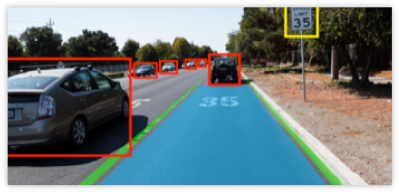
\includegraphics[width=0.9\linewidth]{./img/nvidia_car_detection.png}
      \caption{En la figura se puede observar la detección de objetos que hace el vehículo, utilizando Redes Neuronales Convolucionales en tiempo real}
      \label{fig:car_detection}
    \end{figure}
    \paragraph{Visión por Computadoras}
      El área de Visión por Computadoras es el área de las Ciencias de la Computación que se encarga de cómo las computadoras pueden lograr obtener una comprensión de alto nivel de imágenes digitales o vídeos.
      Desde la perspectiva de la ingeniería, busca automatizar tareas que el sistema visual humano puede hacer. Incluye métodos para adquirir, procesar, analizar y comprender las imágenes del mundo real
      con el fin de producir información numérica o simbólica para que puedan ser tratados por una computadora. El objetivo principal de Visión por Computadoras es reducir la distancia
      entre lo que un humano interpreta a partir de una imagen y la forma en la que las computadoras representan esa misma imagen.

  \section {Motivación}
    En lo que respecta al área de visión por computadoras, una imagen es representada por un arreglo de 2 dimensiones donde cada valor representa la intensidad captada por un sensor
    de un determinado punto espacial, representados como píxeles. La representación de los píxeles es muy sensible a cambios en la iluminación, ángulo, contraste y tamaño que pueda existir.\\
    Además, este tipo de representación es insuficiente para proveerla como dato de entrada de un algoritmo que se encargue de realizar alguna de las tareas antes mencionadas, como la
    detección de objetos o la transferencia de estilos, ya que para estos, es necesario proveer una representación de mas alto nivel, que permita detectar características de alto nivel,
    como formas, contornos, etc. Debido a esto se suelen utilizar representaciones intermedias para este tipo de algoritmos, para el caso del problema de transferencia de estilo,
    al utilizar Redes Neuronales Convolucionales, estas redes aprenden a generar representaciones intermedias de alto nivel, es decir, conceptos dados a nivel semántico.\\
    Existen artículos de investigación en los cuales se definen algoritmos para la transferencia de estilos artísticos en fotografías, que se basan en modelos estocásticos,
    los cuales requieren una gran cantidad de hiper-parámetros predefinidos empíricamente, es decir parámetros que deben ser fijados previo a la ejecución del algoritmo que dependen
    de la elección propia del usuario, pero que influyen en gran manera sobre el resultado. Al ser modelos estocásticos, se basan en la idea de iterativamente,
    minimizar una función de pérdida hasta lograr el objetivo deseado. \\
    El principal objetivo de este trabajo es poder realizar una elección inteligente de uno de los principales hiper-parámetros como lo es el número de iteraciones
    que debe realizar el algoritmo hasta obtener un resultado interesante. \\
    Para poder determinar cuando un resultado logra ser aceptable es necesario definir una métrica para esto.
    Debido a que las obras de arte, sueles calificadas con métricas cualitativas y no tanto cuantitativas, se decidió utilizar otra red neuronal convolucional,
    entrenada especialmente para reconocer estilos artísticos y en base a los resultados que arroja se define si el número de iteraciones es suficiente para generar el resultado final
    o es necesario continuar iterando. \\
    Para introducir al lector en el tema en la figura \ref{fig:style_transfer_candy_tower} se puede observar un ejemplo del resultado de aplicar la transferencia de estilo en fotografias.
    \begin{figure}[h]

      \subfloat[Imagen de Estilo]{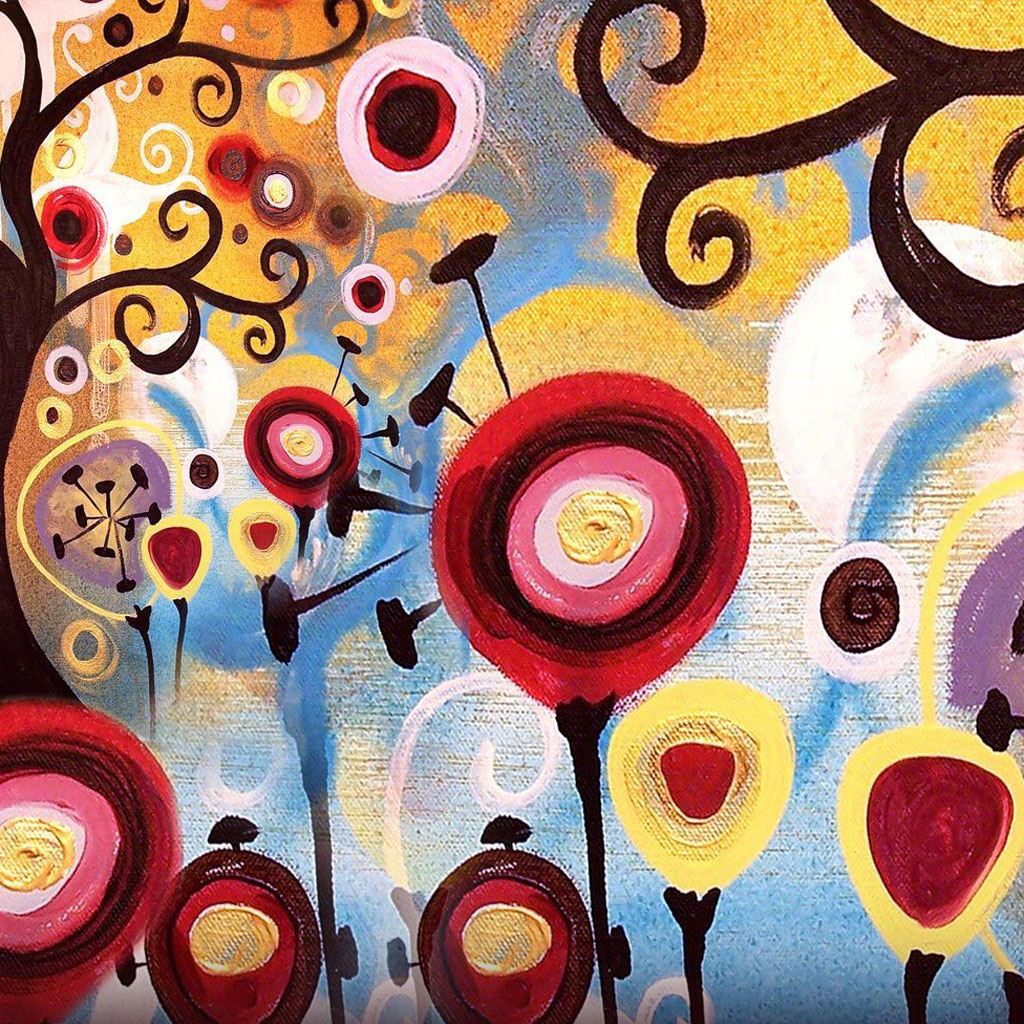
\includegraphics[height=0.3\textheight]{./img/jhonson_style_candy.jpg}\label{fig:candy}}

      \subfloat[Imagen de Contenido]{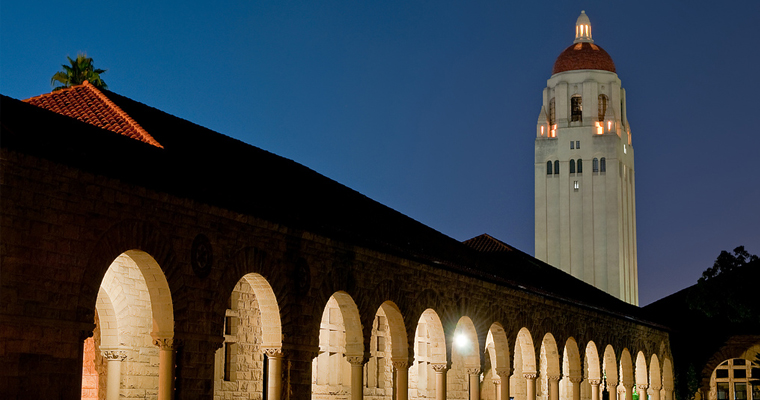
\includegraphics[height=0.3\textheight]{./img/jhonson_content_tower.jpg}\label{fig:tower}}

      \subfloat[Resultado obtenido transfiriendo el estilo de la obra de arte a la imagen de contenido]
      {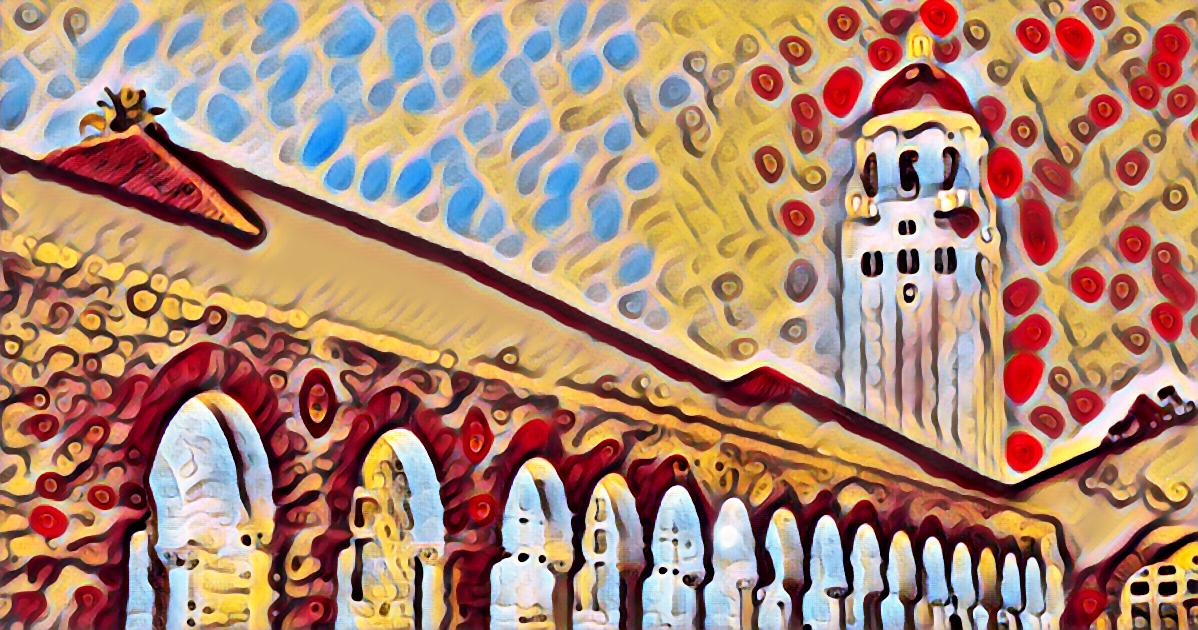
\includegraphics[height=0.3\textheight]{./img/jhonson_result_tower_candy.jpg}\label{fig:candy_tower}}

    \caption{Ejemplo de transferencia de estilo}
    \label{fig:style_transfer_candy_tower}
    \end{figure}

  \section {Estructura del trabajo}
    A lo largo de este trabajo se hará un recorrido por los principales conceptos para comprender tanto el problema como la solución y las técnicas empleadas para la transferencia
    de estilos artísticos en fotografías.\\
    El capítulo 2 se desarrolla el marco teórico y cuestiones formales requeridas, principalmente orientado al aprendizaje Automático y a las redes neuronales.\\
    En el capitulo 3 se hará un recorrido por los principales artículos de investigación y los algoritmos allí definidos para las técnicas de transferencia estilos artísticos en fotografías.
    Para luego, en el capítulo 4 abordar en detalle la solución propuesta, junto con un análisis y evaluación empírica de la misma.\\
    En el capítulo 5 contiene los experimentos realizados y los resultados obtenidos, para finalmente en el capitulo 6 establecer una conclusión acerca del trabajo realizado,
    junto con las perspectivas y posibles tareas a futuro.

\chapter{Marco Teórico}

%Material para revisar
%http://cs231n.github.io/
%Capítulo 2 del Mitchel (1997), Capítulos 3 y 6 del Mitchel (1997)
%Wolpert, D.H., Macready, W.G. (1997), "No Free Lunch Theorems for Optimization," IEEE Transactions on Evolutionary Computation 1, 67
%http://en.wikipedia.org/wiki/Inductive_bias
%http://en.wikipedia.org/wiki/Overfitting
%http://en.wikipedia.org/wiki/SURF
%Capítulo 5 del Marlsand (2009) "Machine Learning, an Algorithmic Perspective"
%Capítulo 5 del Smola & Vishwanathan (2008) "Introduction to Machine Learning"
%http://en.wikipedia.org/wiki/Logistic_regression
%http://en.wikipedia.org/wiki/Linear_regression
%Capítulo 13 del Owen et al. (2012), Capítulo 2 y 4 del Owen et al. (2012)
%http://ufal.mff.cuni.cz/~zabokrtsky/courses/npfl104/html/feature_engineering.pdf
%http://aprendizajengrande.net/cronograma.html
%http://www.deeplearningbook.org/
%Bishop



  \section{Aprendizaje Automático}
    \subsection{Introducción}
      El Aprendizaje Automático (o machine learning, por su denominación en
      inglés) es un campo que se encuentra en la intersección de las ciencias de la computación y el aprendizaje estadístico que le otorga a las computadoras la habilidad de aprender o inferir reglas que no fueron explícitamente programadas.
      Surge desde el estudio de reconocimiento de patrones, y el aprendizaje computacional, provenientes de la Inteligencia artificial, este campo explora el estudio y la construcción de algoritmos
      que pueden aprender y realizar predicciones a partir de datos. En base a las reglas determinadas explícitamente en el programa y los datos de ejemplo, se crea un modelo que intenta predecir
      características de un dato nuevo. Este tipo de algoritmos tienen su enfoque basado en los datos.\\
      Tom M. Mitchell elaboró una definición más formal de este concepto de aprendizaje: “se dice que un programa de computadora aprende de una experiencia E con respecto a una clase
      de tarea T y medición de desempeño P, si su desempeño en la tarea T, medido por P, mejora con la experiencia E” [Mitchell,1997].\\
      El aprendizaje automático es esencialmente una forma de estadística aplicada con énfasis en el uso de computadoras para estimar estadísticamente funciones complicadas.

    \subsection{Clasificación de algoritmos de aprendizaje automático}
      Dentro del aprendizaje automático, los algoritmos se pueden clasificar
      según la forma en la que aprenden a partir del tipo de los datos que le son provistos para su entrenamiento.

      \subsubsection{Aprendizaje Supervisado}
	Los algoritmos de aprendizaje supervisado son, a groso modo, algoritmos de aprendizaje que aprenden a asociar alguna entrada con alguna salida,
	dado un conjunto de entrenamiento de ejemplos que consiste de entradas $x$ y salidas $y$.
	Consisten en aprender una función, a partir de datos de entrenamiento etiquetados. Cada ejemplo del conjunto de entrenamiento suele ser un par
	compuesto de un objeto de entrenamiento (representado por un vector de características) y una etiqueta, que seria el valor de salida deseado.
	A partir de los vectores de características y etiquetas con las que se entrenó, aprende a predecir la etiqueta de un nuevo vector de características nunca antes visto.
	Los problema típicos que se atacan con estos algoritmos son la regresión y la clasificación, dependiendo si la variable a predecir es continua o discreta.

	\paragraph {Regresión}
	  El objetivo de la regresión es predecir el valor de una o más de las variables (continuas) objetivo $t$, dado el valor de un vector $x$ de variables de entrada.
	  Un ejemplo de un problema de regresión sería el de predecir el puntaje crediticio que obtiene un cliente que solicita un préstamo en un banco, donde el vector de entrada
	  consistiría de información financiera, como sueldo, monto disponible en tarjetas de crédito, etc.

	\paragraph {Clasificación}
	  Clasificación se define como el problema de identificar a que categoría (variable discreta) pertenece una nueva observación, basada en el conjunto de datos de entrenamiento,
	  que contiene observaciones a las cuales  si se les conoce categoría. En el escenario más común, las clases o categorías son disjuntas,
	  de modo que cada entrada es asignado a una y sólo una clase. El espacio de entrada es por lo tanto dividido en regiones de decisión, cuyos límites se denominan límites de decisión.
	  Para problemas de regresión, la variable t es simplemente el vector de números reales cuyos valores queremos predecir. En el caso de la clasificación,
	  hay diversas maneras de usar los valores objetivo para representar las etiquetas de clase. En el caso de los dos clase de problemas, es la representación binaria
	  en la que hay un único destino la variable $t \in {0, 1}$ tal que $t = 1$ representa a una clase y $t = 0$ es a la otra.

      \subsubsection{Aprendizaje No Supervisado}
	  Los algoritmos de aprendizaje No Supervisado se caracterizan por aplicarse a conjuntos de datos a los cuales, durante la etapa de entrenamiento no se les conoce su etiqueta
	  de salida, es decir, a diferencia de los algoritmos de aprendizaje supervisado, estos solo disponen del vector de características para el entrenamiento, en lugar de disponer
	  de vectores y etiquetas. Estos algoritmos se emplean para detectar patrones o similaridades entre los datos que eran desconocidas.
	  El principal algoritmo de aprendizaje no supervisado es el de Agrupamiento (Clustering en la literatura en inglés).

	\paragraph {Agrupamiento}
	   El algoritmo de Agrupamiento consiste en reunir objetos en grupos, de forma tal que los objetos pertenecientes a un mismo grupo son en algún sentido mas similares
	   entre ellos que a los objetos que pertenecen a otro grupo. El objetivo de los métodos de agrupamiento es descubrir relaciones significativas presentes en los datos, por lo
	   que el concepto central es la definición de una función de distancia entre las instancias. Cada definición de distancias induce un agrupamiento de los datos, basado en esa métrica.

	  \begin{figure}[h]
	    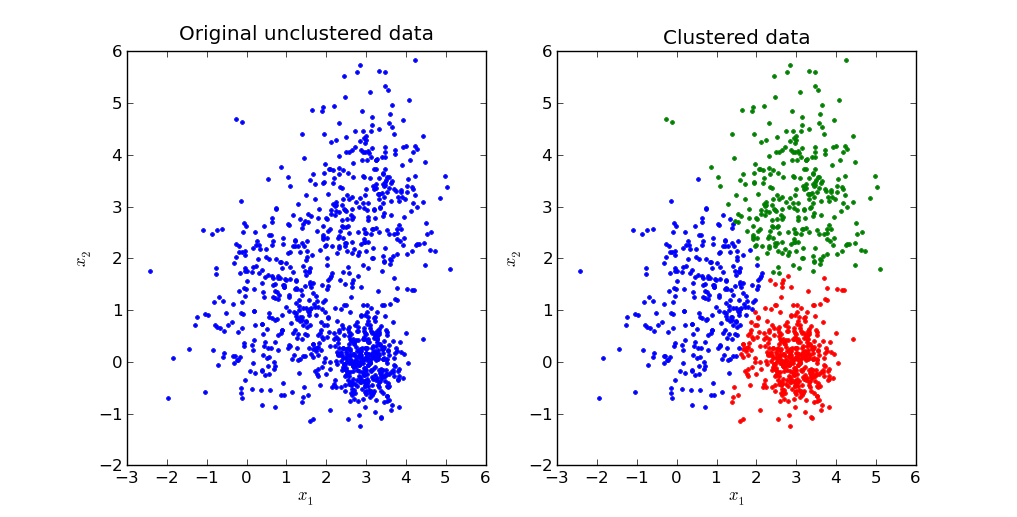
\includegraphics[scale=0.5]{./img/stackoverflow_clustering.png}
	    \caption{En la primer figura se puede observar los datos distribuidos en el espacio, que luego son agrupados por colores en 3 clases distintas}
	    \label{fig:clustering}
	  \end{figure}

      \subsubsection{Aprendizaje Semi-Supervisado}
	Estos algoritmos se caracterizan por utilizar una pequeña cantidad de datos etiquetados y otro gran conjunto de datos no etiquetados
	El principal problema atacado es el de la recomendación.
	\paragraph{Recomendación}
	  El problema de recomendación consiste en tratar de predecir la preferencia que un usuario podría hacer por un artículo. Los sistemas de recomendación se han convertido cada
	  vez más populares en los últimos años, y se pueden utilizar en una variedad de áreas, incluyendo películas, música, noticias, libros y productos en general.
	  El enfoque mayormente utilizado es el de filtrado colaborativo, que se basa en la recolección y el análisis de una gran cantidad de información sobre los usuarios,
	  los comportamientos, actividades o preferencias y la predicción de lo que los usuarios tendrán como base en su similitud con otros usuarios.

      \subsubsection{Aprendizaje por Refuerzo}
	El sistema interactúa en un ambiente dinámico en el cual debe cumplir un objetivo determinado, el programa va recibiendo retroalimentación en términos de premios y castigos mientras
	recorre el espacio del problema y de esta forma aprende.\\
	El aprendizaje de refuerzo difiere del aprendizaje supervisado en que nunca se presentan pares de entrada/salida correctos, ni acciones subóptimas corregidas explícitamente.
	Además, se hace hincapié en el rendimiento en tiempo real, que consiste en encontrar un equilibrio entre la exploración (del territorio desconocido) y la explotación
	(del conocimiento actual).
	Por ejemplo, mediante aprendizaje por refuerzo una computadora puede aprender a jugar al Backgammon o al Ajedrez a niveles profesionales.

    \subsection{Vectores de Características para el Aprendizaje}
      \FIXME{Posible Referencia \url{http://machinelearningmastery.com/discover-feature-engineering-how-to-engineer-features-and-how-to-get-good-at-it/}}
      Para que un modelo pueda aprender, es necesario definir un vector de características (features vector en inglés) que este deberá aprender a partir de las instancias de entrenamiento.
      Una Feature es una pieza de información que podría ser útil para la predicción. Cualquier atributo podría ser una feature, siempre y cuando sea útil para el modelo.
      Según el tipo de dato, las características irán variando. \\
      Por ejemplo para representar un documento de texto, el método mas utilizado es la bolsa de palabras.
      Este método genera una característica por cada palabra de su vocabulario, y cada documento es representado por un vector, cada posición del vector se asocia a una palabra del
      vocabulario y el valor que posee esa posición es la cantidad de veces que aparece la palabra asociada.

      \subsubsection{Representando imágenes}
	Es un campo de investigación que en la actualidad se encuentra muy activo. El método más sencillo es usar el valor de los píxeles directamente, aunque este no generaliza muy bien
	Pero puede mejorar utilizando transformaciones algorítmicas del conjunto de entrenamiento el siguiente paso seria tomar el promedio sobre pequeños cuadrados de la imagen.
	Necesitamos de alguna función compleja que comprenda el significado de la imagen más allá de la representación numérica de la misma.
	A lo largo del desarrollo de la visión por computadora se distinguen dos enfoques para la generación de descriptores capaces de reconocer características de una imagen:
	El enfoque basado en técnicas superficiales (o “shallow” en inglés) y el enfoque de aprendizaje profundo (o “deep” en inglés).

      \subsubsection{Enfoque Clásico}
	El enfoque clásico (Shallow en la literatura en ingles) responde a la manera tradicional de hacer visión por computadoras. Se busca generar una representación invariante
	a la posición, iluminación, fondo, etc. utilizando principalmente técnicas estadísticas a partir de conocimiento anterior del objeto y del contexto.
	Los descriptores son diseñados a mano a partir de características físicas, hipótesis y observaciones. Con este enfoque no se aprenden características de los objetos sino que
	se procesa la imagen de interés con un extractor de features prefijadas y luego se pasa la nueva representación a un clasificador entrenable.
	Los métodos más utilizadas que generan este tipo de descriptores son SIFT, SURF y Vectores Fisher.
	Otro ejemplo es el de la bolsa de palabras visuales, similar al método ejemplificado para texto, que se ilustra en la siguiente imagen:\\
	\begin{figure}[h]
	  \begin{center}
	    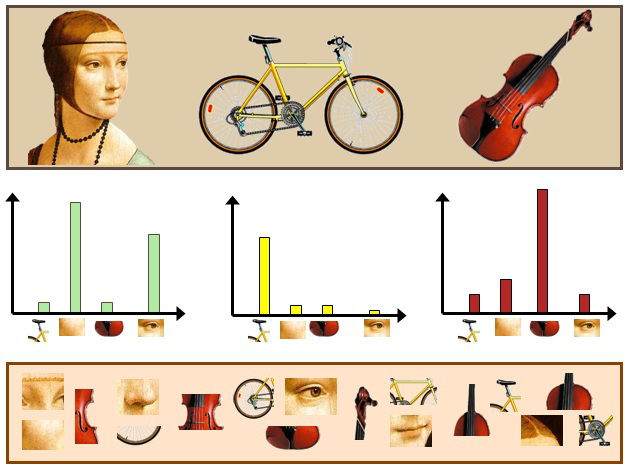
\includegraphics[scale=0.5]{./img/bag_of_visual_words.jpg}
	    \caption{Ejemplo de Bolsa de Palabras visuales}
	  \end{center}
	  \label{fig:bovw}
	\end{figure}

	Estas técnicas son utilizadas como paso de preprocesamiento de la imagen, ya que representación cruda en píxeles es insuficiente para proveerla como dato de entrada de un algoritmo
	de aprendizaje automático ya que para estos, es necesario proveer una representación de mas alto nivel, que permita detectar características de alto nivel,
	como formas, contornos, etc. Es decir que provean una especie de contenido semántico de la imagen.

      \subsubsection{Enfoque de Aprendizaje Profundo}
	En este enfoque tiene como objetivo lograr representar el contenido semántico de una imagen mediante un único algoritmo que aprenda a representarlo por si mismo,
	a partir de los datos, 	en lugar de que sean diseñadas a mano y prefijadas en el detector.
	El problema asociado a esto es que no sabemos cuales serán las features que el modelo aprende durante el entrenamiento y tampoco se logran comprender claramente.
	Lo que si se conoce es que las features aprendidas tienen en cierto modo una especie de jerarquía, es decir que las features de bajo nivel aprendidas desde los píxeles
	alimentan el aprendizaje de otras features que aprenden a reconocer contornos y bordes, y así sucesivamente hasta llegar a las features de mas alto nivel que logran reconocer
	estructuras y objetos. Debido a esto, las estructuras de aprendizaje profundo contemplan esta particularidad organizándose en diferentes capas, donde la salida de una capa
	es la entrada a la capa siguiente. Las Redes Neuronales Convolucionales soportan el aprendizaje de este tipo features y es el modelo que analizaremos posteriormente en este trabajo.\\
	\begin{figure}[h!]
	  \begin{center}
		  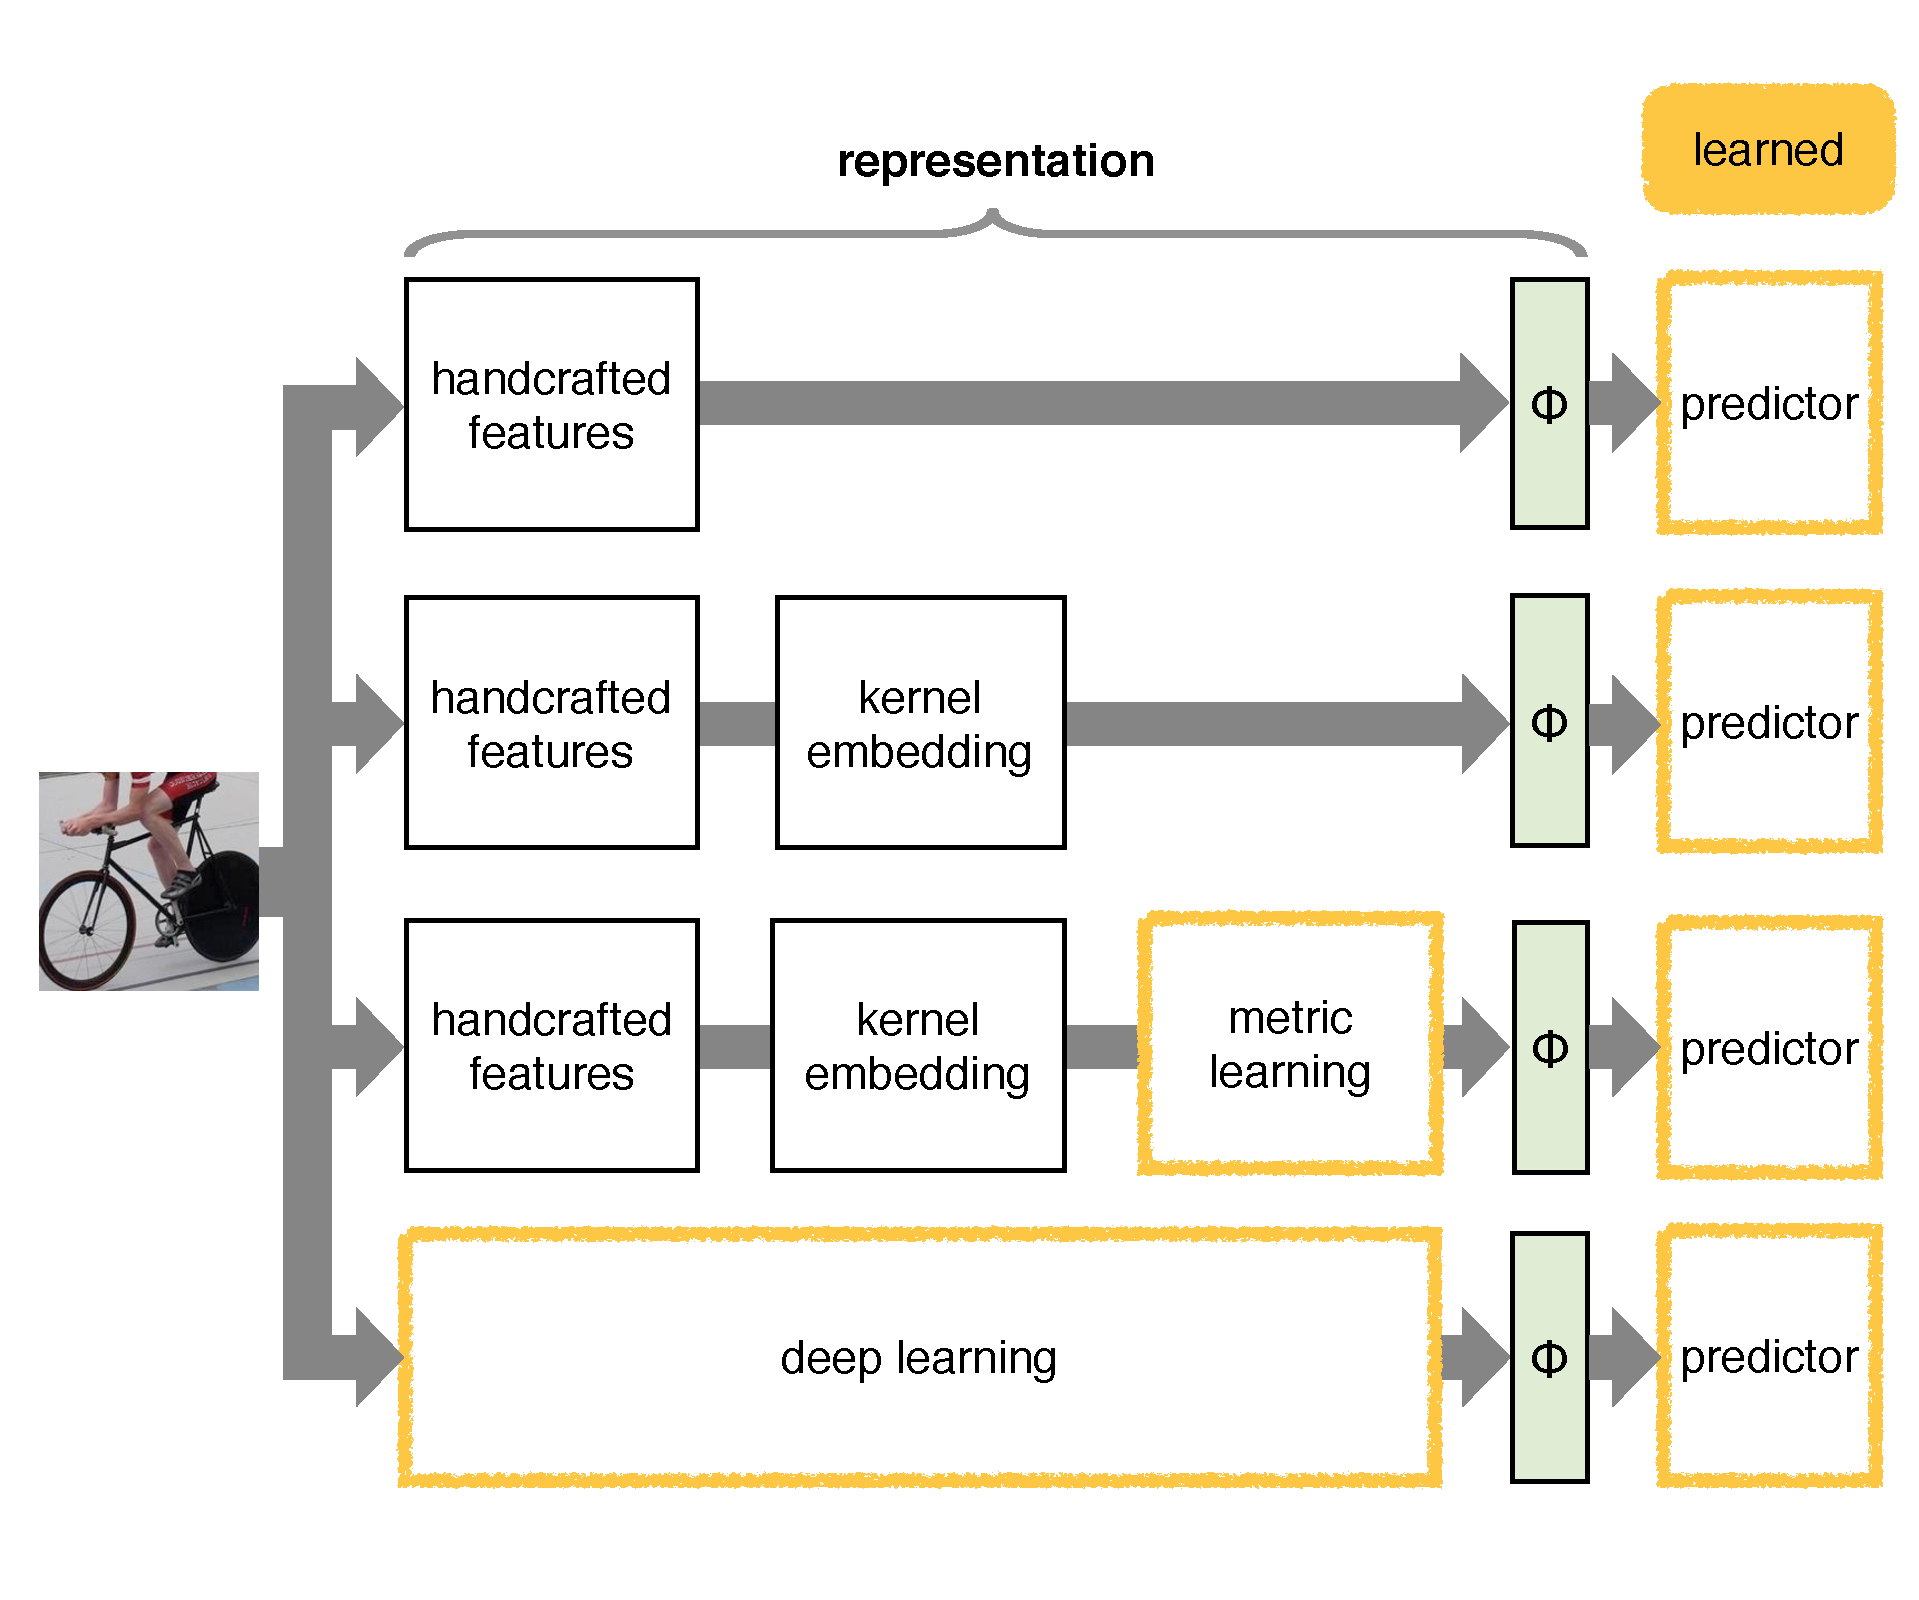
\includegraphics[width=0.9\linewidth]{./img/vedaldi_shallow_deep.pdf}
	  \caption{En las 3 primeras opciones del diagrama se pueden observar las distintas formas de representar imágenes mediante técnicas de aprendizaje automático tradicional,
	  donde las características deben estar predefinidas a mano, en cambio para las técnicas de aprendizaje profundo, las representaciones son aprendidas durante el entrenamiento
	  del modelo.}
	  \label{fig:shallow_deep}
	  \end{center}
	\end{figure}

      \subsection{Entrenamiento}
	A continuación detallaremos algunos conceptos principales para el entrenamiento de un modelo y luego se explica como funciona la fase de aprendizaje.
	\subsubsection{Función de Predicción \label{sec:prediccion}}
	  Una predicción puede tener un resultado binario (0 o 1) o puede devolver un puntaje por lo general con valores continuos entre 0 y 1, indicando un cierto valor de confianza
	  de la predicción. Para el caso de un problema de clasificación de imágenes, el modelo dado una imagen, puede otorgar un puntaje a cada una de las $K$ clases posibles,
	  y la que obtenga el mayor puntaje será la clase asignada para esa imagen. Para poder realizar una predicción es necesaria una función de puntuación $f:R^D {\rightarrow} R^K$
	  donde $D$ es la dimensionalidad del vector de entrada que toma $f$. \\
	  Además, es necesario una función de decisión $H$, por ejemplo para el caso de clasificación $H:R^K{\rightarrow}{1,..,K}$
	  que toma el resultado de $f$ y decide a cual de las $K$ clases pertenece y para el caso de la regresión es la función identidad $H(f(x))=f(x)$.
	  Un ejemplo de función de puntuación:
	  Suponiendo que tenemos $x$ una imagen de entrada, que la queremos asociar a una clase $y_{j}$ de las $K$ clases posibles , sea $D$ la dimensionalidad de $x$, $x \in R^D$,
	  $j \in 1..K$, entonces $f$ es una función: $f:R^D {\rightarrow} {1,..,K}$. El caso mas simple es el de una clasificador lineal:\\
	  \begin{equation}
	    f(x, W, b) = W x + b
	  \end{equation}
	  Donde $W \in R^{K \times D}$, $b \in R^{K \times 1}$ son los parámetros de la función. $W$ suele ser llamado los pesos y $b$ el sesgo, ya que influye en el resultado de salida, pero sin
	  interactuar con el dato de entrada.
	  Algunas cosas a tener en cuenta:
	  \begin{itemize}
	   \item Observar también que consideramos los datos de entrada $(x, y_{j})$  prefijados, pero tenemos control sobre el ajuste de los parámetros $W$ y $b$.
		 Nuestro objetivo será establecerlos de tal manera que las puntuaciones computadas coincidan con las etiquetas correctas sobre todo conjunto de entrenamiento.
		 Intuitivamente deseamos que la clase correcta tenga una puntuación más alta que las puntuaciones de las clases incorrectas.
	   \item Una ventaja de este enfoque es que los datos de entrenamiento se utilizan para aprender los parámetros $W$ y $b$, pero una vez que el aprendizaje es completo,
		podemos descartar el conjunto de entrenamiento completo y sólo mantener los parámetros aprendidos. Esto se debe a que una nueva imagen nunca vista puede ser
		simplemente reenviada a través de la función y clasificada en base a las puntuaciones computadas.
	  \end{itemize}
	  \begin{figure}[h!]
	    \begin{center}
	     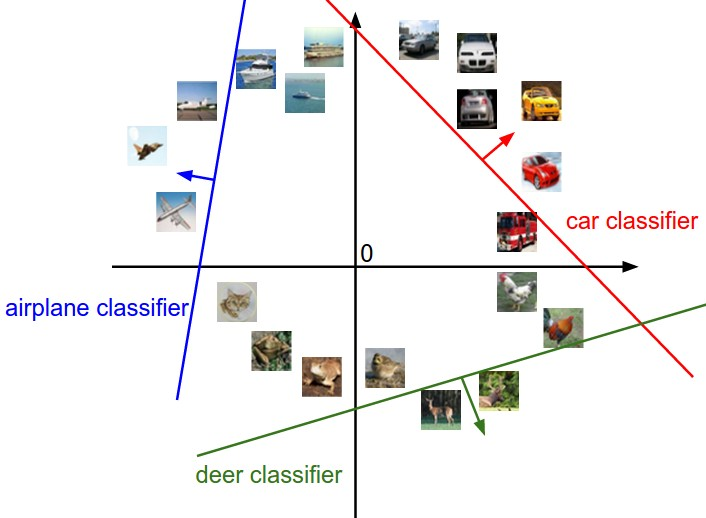
\includegraphics[scale=0.5]{./img/stanford_linear_class.jpeg}
	    \end{center}
	    \caption{Ejemplo de clasificador lineal que utiliza una función de puntuación lineal para clasificar entre autos, aviones y ciervos}
	    \label{fig:figure2}
	  \end{figure}

	\subsubsection{Funciones de Pérdida}
	  El problema de estimar los parámetros de un modelo, se resuelve optimizando una función de costo que se puede expresar como:
          \begin{equation}
	    L = \frac{1}{N}\sum_{i=1}^{N} L_i(y_i, f(x_i, W, b)) + \lambda \Omega(W)
          \end{equation}
          Con $L:\mathcal{Y}\times \mathcal{Y}\rightarrow\mathbb{R}_+$, donde $\mathcal{Y}$ en el caso de la clasificación de la Sec.~\ref{sec:prediccion} seria ${1,..,K}$.
          Esta ecuación contiene 2 términos: Un termino relacionado a las funciones de pérdida de cada imagen $L_i(y_i, f(x_i, W, b))$
          y un coeficiente de regularización $\lambda \Omega(W)$ que penaliza a los modelos complejos, $\lambda$ es un hiper-parámetro que define cuanto influye la regularización
          sobre el resultado final y $N$ es la cantidad de datos de entrenamiento.
	  Una función de pérdida es una función real, no negativa $L({\widehat y}, y)$, que mide cuán diferente es la predicción ${\widehat y}$ obtenida, con respecto a la
	  salida esperada $y$. Existen diversas funciones de pérdida que se utilizan en distintos contextos. A continuación se presentan algunas que se aplican usualmente:
	  \begin{itemize}
	    \item Función de Pérdida 0-1:
	      \begin{equation*}
		L({\widehat y}, y) =  \begin{cases}
					    1 \text{si ${\widehat y} = y$}
					    0 \text{en caso contrario.}
		                      \end{cases}
	      \end{equation*}
	    \item Función de Pérdida Hinge:
	      \begin{equation*}
		L({\widehat y}, y) =  max(0, 1 - {\widehat y}y)
	      \end{equation*}
	      Ampliamente utilizada para algoritmos de Maquina de Vector Soporte.
	      Es una función convexa y continua pero no es derivable por lo tanto no se puede utilizar en métodos como el Descenso por el Gradiente.
	    \item Función de Pérdida Logística:
	      \begin{equation*}
		L({\widehat y}, y) =  {\log(1+ {\exp^{-{\widehat y}y}})}
	      \end{equation*}
	      Similar a la función Hinge, pero al ser derivable, puede utizarse para aplicar Descenso por el gradiente.
	    \item Función de Pérdida de Entropía Cruzada
	      \begin{equation*}
		L({\widehat y}, y) = -y{\log({\widehat y}}) - (1-y) {\log(1-{\widehat y})}
	      \end{equation*}
	      Es una función continua, convexa y derivable que se adapta a métodos de Descenso por el gradiente, se utiliza en Redes Neuronales Profundas.

	  \end{itemize}

	\subsubsection {Sobreajuste y Regularización}
	  Uno de los principales objetivos de los algoritmos de aprendizaje automático es su capacidad de generalizar a ejemplos nunca antes vistos. Sin embargo, si la fase
	  de aprendizaje se realiza durante demasiado tiempo o si los ejemplos del conjunto de entrenamiento son raros, el modelo aprendido podría ajustarse específicamente
	  a ciertas características aleatorias de estos datos, que en realidad no contribuyen a la generalización. Esto se conoce como sobreajuste (overfitting en la literatura en inglés),
	  y es un problema importante y ampliamente discutido en el campo de aprendizaje automático. En el proceso de sobre ajuste, el desempeño del algoritmo en el
	  conjunto de entrenamiento sigue mejorando, pero en el conjunto de evaluación empeora.\\
	  Una técnica para evitar el sobre ajuste de modelos es utilizar regularización. Esencialmente, consiste en penalizar los parámetros del modelo para evitar su
	  crecimiento desmedido, agregando un regularizador($\Omega(W)$) a la Función de Pérdida. \\
	  La función de regularización mas comúnmente utilizada es la norma $L2$, definida como:
	   \begin{equation}
	    \Omega(W) = \frac{1}{2} {\sum_{k} {\sum_{l}} W_{k,l}^2}
	   \end{equation}

    \subsubsection{Optimización}
      Minimizar la función de pérdida puede considerarse un problema de optimización, con lo cual se pueden aplicar las técnicas empleadas en este tipo de problemas, para resolverlo.
      El objetivo de la optimización es encontrar el vector de pesos $W$ que minimice la función de pérdida.\\
      La estrategia de optimización mas utilizada para este tipo de problemas es la de seguir la dirección del gradiente (también llamado derivada) de la función de pérdida.
      En este caso que la función toma como entrada un vector de números, se aplican las derivadas parciales y el gradiente es el vector resultante de calcular las derivadas parciales
      en cada dimensión.La idea de principal de este método es el refinamiento iterativo, se evalúa el resultado del calculo del gradiente y se actualizan los parámetros repetidamente,
      toma un hiper-parámetro $\eta$ llamado tasa de aprendizaje que define el tamaño de cada paso en la iteración.
      Sea $F$ la función de pérdida, $w$ el vector de pesos, $N$ el numero de datos de entrenamiento, cada iteración consiste de:

      \begin{equation}
	w_{n+1} = w_n - \eta \nabla L(w_n)  = w_n - \eta \sum_{i=1}^{N} \nabla L_i(w_n)
      \end{equation}

      Un problema recurrente en el aprendizaje automático es que para una buena generalización, son necesarios grandes conjuntos de entrenamiento,
      pero grandes conjuntos de entrenamiento también son más costosos desde el punto de vista computacional.
      En aplicaciones de gran escala, el conjunto de entrenamiento puede ser del orden de los millones de ejemplos, por lo que computar la función de
      pérdida completa sobre todo el conjunto para actualizar un solo parámetro seria algo impracticable.\\
      Un enfoque común que se aplica a este problema es computar el gradiente sobre pequeños lotes del conjunto de entrenamiento,
      que permite lograr una buena aproximación al objetivo completo con una convergencia mucho mas rápida, es decir se reduce $N$ a un pequeño subconjunto, de esta forma se
      reduce el numero de cálculos realizados en cada iteración. Este método se lo conoce como \emph{Descenso por el gradiente estocástico} y es el mas utilizado para optimizar
      funciones de pérdida en las Redes Neuronales.

	\begin{algorithm}[H]
	  \caption{Descenso por el gradiente estocástico}
	  \label{SGD}
	  \begin{algorithmic}
	    \State Elegir una tasa de aprendizaje $\eta$
	    \State Elegir un vector de pesos inicial $w_0$
	    \State Elegir un numero de iteraciones $J$
	    \State Ordenar aleatoriamente
	    \State $w \gets w_0$
	    \For{$j=1,..J$}
	      \ForAll {$i=1,..,N$}
		$sum_{gradiente} \gets sum_{gradiente} + \nabla L_i(w_n)$
	      \EndFor
	      \State $w \gets w - \eta sum_{gradiente}$
	    \EndFor
	  \end{algorithmic}
	\end{algorithm}

    \subsection{Ciclo del Aprendizaje Automático}
      Luego de explicar todos los conceptos relevantes al Aprendizaje automático, podemos resumir al ciclo común a todos los algoritmos de Aprendizaje automático a lo siguiente:
      \begin{enumerate}
	\item Recopilación de datos:
	  El recopilado de datos es crucial, puede requerir mucho esfuerzo y cambio de procesos complejos,
	  Anotación, Muchas veces la clase objetivo tiene que ser calculada a mano por grupos de personas designadas para la tarea.
	\item Preprocesamiento de datos: Una vez obtenidos los datos, es necesario preprocesarlos para lograr tener datos limpios y útiles. Esta fase puede contener una etapa
	  de exploración y análisis, la cual permite conocer el dominio de donde provienen los datos.
	\item Definición de características: Para definir las características que el modelo debe aprender, en muchas ocasiones es necesario tener conocimiento del dominio a partir del cual provienen los datos.
	  La ingeniería de features ayuda a obtener características que provean información relevante a la hora de predecir.
	\item Entrenamiento:
	  \subitem Antes de comenzar el entrenamiento el conjunto de datos se divide en 2 subconjuntos, un conjunto de datos de entrenamiento y un conjunto de datos de prueba.
	  \subitem Para entrenar el modelo solo se utiliza el conjunto de datos de entrenamiento, el conjunto de datos de prueba se separa.
	  \subitem Determinar la estructura del modelo de aprendizaje, en base al tipo de problema y a la forma en la que se representan las características de los datos.
	  \subitem En algunos modelos, a partir del conjunto de datos de entrenamiento, se realiza otra partición de un pequeño subconjunto llamado conjunto de datos de validación, este conjunto sirve
	  para afinar ciertos hiper-parámetros del modelo.
	  \subitem Entrenar el modelo elegido sobre el conjunto de datos de entrenamiento
	\item Evaluación: Se aplica el modelo entrenado a los datos del conjunto de prueba, y se aplican métricas para poder establecer que tan bien predice el modelo entrenado para datos nunca antes vistos.
      \end{enumerate}

\iffalse

    \section{Clasificación de imágenes mediante Aprendizaje
      Supervisado}\FIXME{REMOVE. DEJARLO EN SUSPENSO PARA VER DONDE VA MÁS ADELANTE}
      \subsection{Introducción}
	La clasificación de imágenes es un problema que consiste en asignar a una imagen de entrada, una etiqueta de categoría a partir de un conjunto prefijado de categorias.
	Es uno de los principales problemas del area de visión por computadoras, pero que a pesar de su simplicidad tiene una gran cantidad y variedad de aplicaciones practicas,
	al punto de que otros problemas provenientes del area de visión por computadores pueden ser como detección de objetos o segmentacion pueden ser reducidos a clasificación de imágenes.
	El objetivo de presentar este problema es motivar el uso de las redes neuronales convolucionales en las siguientes secciones.
	\begin{figure}[h]
	  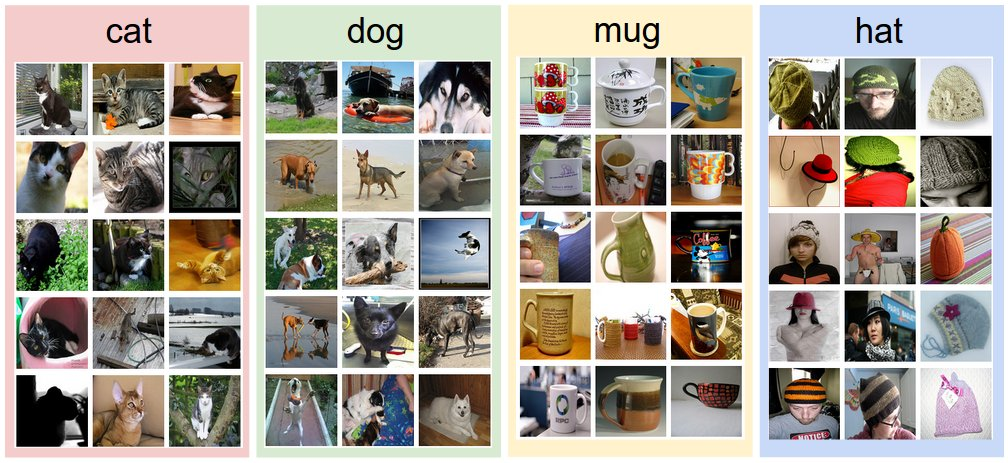
\includegraphics[scale=0.5]{./img/stanford_img_class.jpg}
	  \caption{Clasificación de imagenes en categorias: Perros, Gatos, Tazas y Gorros}
	  \label{fig:stanford_img_class}
	\end{figure}

	\subsubsection {Desafios}
	  Debido a que la tarea de reconocer un concepto visual es relativamente trivial para que lo realice una persona, vale la pena considerar los desafios involucrados desde la perspectiva de
	  un algoritmo de Visión por computadoras, teniendo en cuenta que la representacion pura de una imagen es un arreglo de 3 dimensiones que contiene valores de brillo. A continuacion de mencionan
	  algunos de los principales desafios
	  \begin{itemize}
	    \item Variación del punto de vista: Una simple instancia de un objeto puede estar orientada de muchas formas frente a la camara que toma la imagen.
	    \item Variación de escala: Las clases visuales suelen exhibir variaciones en su tamaño en el mundo real y no solo en lo referido a la imagen.
	    \item Deformación: Muchos objetos de interes no tienen un cuerpo rigido y pueden ser deformados de muchas formas
	    \item Oclusión: Los objetos de interes pueden estar ocluidos y solo una pequeña porcion del objeto puede ser visible.
	    \item Condiciones de iluminación: Los efectos de la iluminación pueden influir de forma drástica a nivel de píxeles.
	    \item Influencia del fondo: los objetos de interés pueden estar inmersos en un ambiente en el cual sean dificiles de identificar.
	    \item Variaciones intra clase: Existen muchos instancias completamente distinta de una misma categoría de objetos.
	  \end{itemize}
	  Un buen modelo de clasificación de imágenes debe ser tolerante a todos estos desafios presentados.
	  \begin{figure}[h]
	    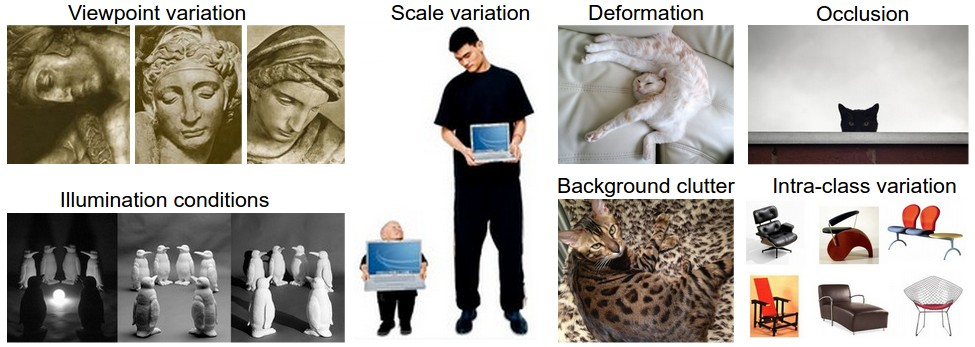
\includegraphics[scale=0.5]{./img/stanford_challenges.jpeg}
	    \caption{Aqui se pueden observar graficamente los desafios enumerados anteriormente}
	    \label{fig:stanford_challenges}
	  \end{figure}

	\subsubsection {Ciclo de Clasificación de Imágenes}
	  \begin{itemize}
	    \item Conjunto de datos de entrada: El conjunto de datos de entrada es un conjunto de N imágenes, cada una etiquetada con una de las K diferentes categorias.
	    \item Aprendizaje: En base al conjunto de datos de entrenamiento, el sistema debe aprender como identificar las caracteristicas de cada categoría para asi establecer un modelo clasificador.
	    \item Evaluación: Finalmente se evalua la calidad del modelo clasificador haciendo que prediga las etiquetas para un conjunto (de prueba) nuevo de imágenes que no habia visto antes, comparando las
	    etiquetas correctas con las etiquetas predecidas por el clasificador se puede establecer una metrica de calidad, intuitivamente se espera que las etiquetas predecidas coincidan en la mayoria
	    de los casos con las etiquetas correctas.
	  \end{itemize}
\fi


    \subsection{Construyendo un algoritmo de aprendizaje automático}
      Casi todos los algoritmos de aprendizaje profundo pueden ser descritos como casos particulares de una receta bastante simple:
      combinar una especificación de un conjunto de datos, una función de pérdida, un procedimiento de optimización y un modelo.
      Al darnos cuenta de que podemos reemplazar cualquiera de estos componentes en gran medida independientemente de los otros, podemos obtener una gran variedad de algoritmos.
      La función de costos incluye típicamente al menos un término que hace que el proceso de aprendizaje realice una estimación estadística. También puede incluir términos adicionales,
      como los términos de regularización. Esto todavía permite la optimización de forma cerrada.
      Si cambiamos el modelo para que no sea lineal, entonces la mayoría de las funciones de pérdida ya no pueden ser optimizadas en forma cerrada.
      Esto nos obliga a elegir un procedimiento iterativo de optimización numérica, como el descenso por el gradiente.

    \section{Redes Neuronales Artificiales}

      \subsection{Introducción}
	Las Redes Neuronales Artificiales básicamente son una combinación lineal de funciones no lineales.
	Un algoritmo de aprendizaje de red neuronal artificial (ANN), usualmente llamado "red neuronal" (NN), es un algoritmo de aprendizaje que se inspira en la estructura y aspectos funcionales
	de la redes neuronales biológicas. Los cálculos se estructuran en términos de un grupo interconectado de neuronas artificiales, procesando la información utilizando un enfoque de grafos
	a la computación. Las redes neuronales modernas son herramientas no lineales de modelado de datos estadísticos. Usualmente se usan para modelar relaciones complejas entre entradas y salidas,
	para encontrar patrones en los datos, o para capturar la estructura estadística en una distribución de probabilidad conjunta desconocida entre las variables observadas. \\
	Las redes neuronales se pueden modelar como un conjunto de neuronas conectadas en un grafo acíclico, que se suelen organizar por capas, las neuronas de una capa
	se conectan con neuronas de sus capas adyacentes pero nunca se conectan 2 neuronas de una misma capa, como se puede observar en la figura \ref{fig:neural_network}.
	Toda red neuronal tiene una capa de entrada, una capa de salida y un número determinado de capas ocultas, que pueden ser de distintos tipos.
	Una de las principales razones por la cual las redes neuronales están organizadas en capas, es que este tipo de estructura permite evaluar una red, muy simple y eficientemente realizando
	operaciones matriciales vectoriales, una red neuronal puede ser pensada como una serie de multiplicaciones de matrices entrelazadas con funciones de activaciones no lineales.
	Las redes neuronales utilizadas en la actualidad tienen alrededor de 100 millones de parámetros distribuidos entre 10-20 capas.
	\begin{figure}[H]
	  \begin{center}
	    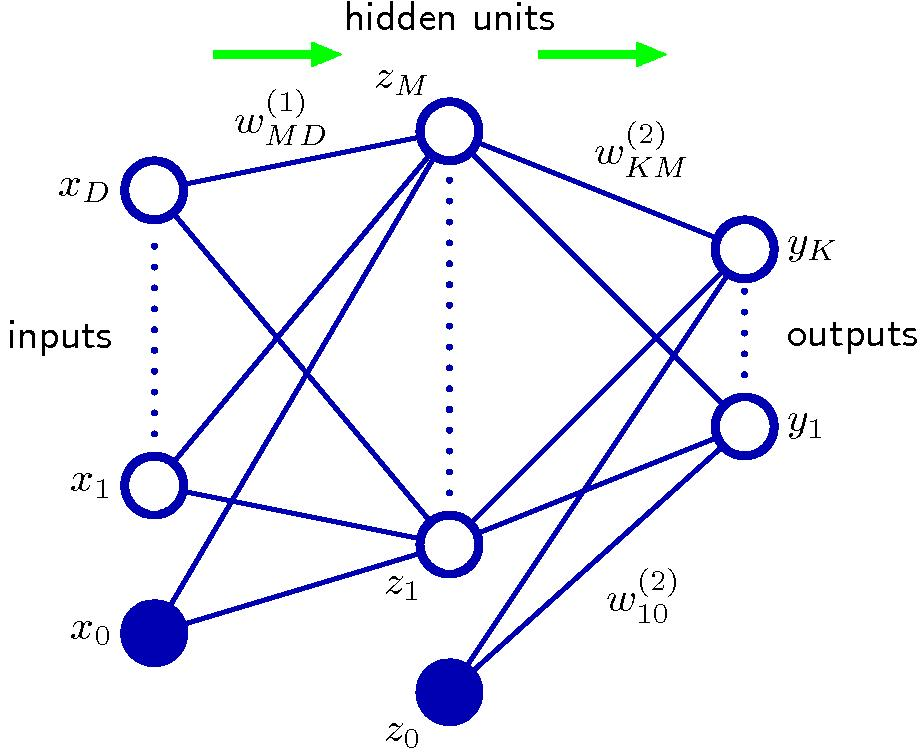
\includegraphics[scale=0.5]{./img/bishop_neural_network.jpg}
	  \end{center}
	  \caption{Red Neuronal Artificial}
	  \label{fig:neural_network}
	\end{figure}

      \subsection{Aprendizaje basado en el Gradiente}
	El diseño y entrenamiento de una red neural no es muy diferente de la formación de cualquier otro modelo de aprendizaje automático con descenso por el gradiente.
	La diferencia más grande entre los modelos lineales y las redes neuronales es que la no linealidad de una red neuronal hace que las funciones de pérdida
	más interesantes se vuelvan no convexas. Esto significa que las redes neuronales suelen ser entrenadas mediante el uso de optimizadores iterativos basados ​​en gradientes
	que simplemente minimizan la función de costo, en lugar de los solucionadores de ecuaciones lineales usados ​​para entrenar modelos de regresión lineal. Para el caso de las
	redes neuronales, la técnica ampliamente utilizada es la de retropropagación del error:

	\subsubsection{Retropropagación del Error}
	  \FIXME{\url{http://cs231n.github.io/optimization-2/} AGREGAR FORMALIDADES REGLA DE LA CADENA}
	  Retropropagación (en inglés Backpropagation) una forma  de computar los gradientes de expresiones mediante la aplicación recursiva de la regla de la cadena.
	  El ciclo consta de 2 fases, propagación y luego actualización de parámetros. Cuando ingresan los parámetro a la función se calcula el resultado final, y se lo compara con el resultado
	  deseado, aplicando la función de pérdida se calcula el error, mediante el método de optimización se define el gradiente para luego realizar la retropropagación en la función hasta
	  actualizar los parámetros.
	  \FIXME{VER EN BISHOP pag 260}
	\subsubsection {Entrenamiento}
	  El entrenamiento de una red neuronal consiste de 2 pasos: paso hacia adelante, y paso de retropropagación del error
	  \begin{enumerate}
	    \item En el paso hacia adelante se evalúa la red y se obtiene el resultado de salida, el cual se mide el error, se calcula el gradiente para luego aplicar el paso de retroalimentación
	    \item En el paso de retropropagación del error se ajustan los pesos internos de la red en base al resultado del gradiente, desde las capas finales de la red hasta las capas iniciales.
	  \end{enumerate}
	  \FIXME{VER EN BISHOP}
	  \begin{figure}[H]
	    \begin{center}
	    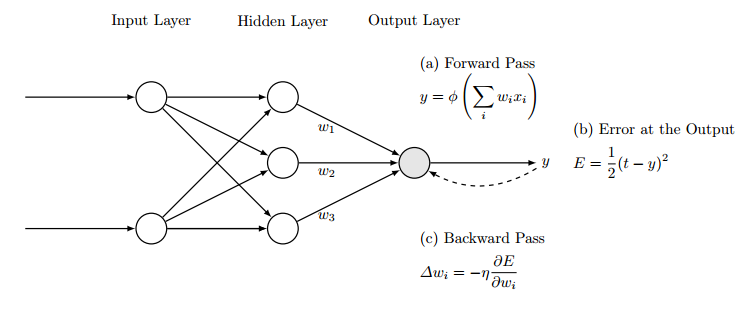
\includegraphics[width=\linewidth]{./img/backprop.png}
	    \end{center}
	    \caption{ Descripción de la retropropagación. (a) El entrenamiento es alimentado hacia delante, generando de salida correspondiente. (b) Error entre la salida real y la salida deseada
	    se calcula. (c) El error se propaga hacia atrás, a través de actualizaciones donde una proporción del gradiente ($ \frac{\partial E}{\partial w_i}$ ) es la resta de cada peso. $x_i$, $w_i$, $\phi$ son las entradas,
	    la entrada de pesos, y la función de activación de una neurona. Error $E$ se calcula a partir de la salida $y$ de salida deseado $t$. $\eta$ es la tasa de aprendizaje.
	    \cite{Automatic_differentiation_ML} }
	    \label{fig:backprop}
	  \end{figure}


      \subsection {Neurona artificial}
	\begin{figure}[H]
          \begin{center}
            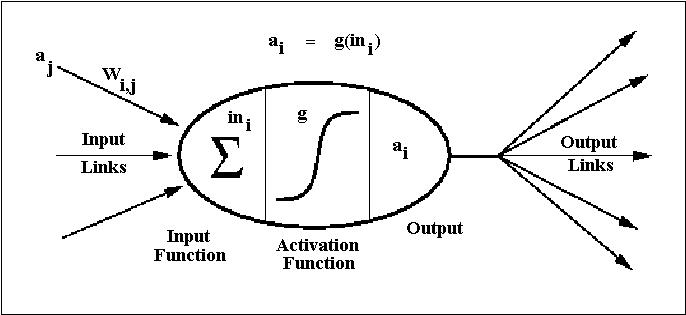
\includegraphics[width=0.4\linewidth]{./img/neuron.jpg}
	  \caption{Neurona artificial \label{fig:neuron}}
          \end{center}
	\end{figure}
	La unidad de procesamiento de una red neuronal es una neurona. La misma consta de un vector de entrada, un vector de pesos y una función de activación no lineal,
	como se puede ver en la figura \ref{fig:neuron}.
	En una neurona se realiza el producto punto entre el vector de entrada, y su vector de pesos, le suma el sesgo y aplica la función no lineal.
	Una única neurona puede ser utilizada para implementar un clasificador binario.


      \subsection {Funciones de Activación comúnmente utilizadas}
	Toda función de activación toma un único número como entrada, realiza un operación matemática predefinida, no lineal y devuelve el resultado obtenido.
	Algunos ejemplos de funciones que se utilizan:
	  \subsubsection {Sigmoide}

	    La función sigmoide proyecta el dominio al rango (0,1) y su ecuación es:
	    \begin{equation*}
	     f(x) = \frac{1}{1+\exp{-x}}
	    \end{equation*}
	    Ha tenido un uso frecuente desde el punto de vista histórico, ya que tiene una interpretación similar a la tasa de activación de una neurona:
	    de no activarse en absoluto (0) a activarse completamente a una frecuencia máxima asumida (1), como puede observarse en la figura \ref{fig:sigmoid}. En la práctica, la función sigmoide recientemente ha dejado de utilizarse,
	    ya  que tiene dos inconvenientes principales:
	    \begin{itemize}
	     \item Se satura y anula el gradiente. Una propiedad muy indeseable de la sigmoide es que cuando la activación de la neurona se satura en cualquiera de las dos puntas de 0 o 1,
	      el gradiente en estas regiones es casi cero.
	     \item Las salidas no están centradas en cero. Esto es indeseable ya que las neuronas en capas posteriores de procesamiento en una Red Neuronal estarían recibiendo
	      datos que no están centrados en cero. Esto tiene implicaciones en la dinámica durante el descenso del gradiente, porque si los datos que llegan a una neurona
	      son siempre positivos, entonces el gradiente en los pesos durante la retropropagación o bien serán todos positivos o todos negativos.
	    \end{itemize}
	    \begin{figure}[H]
	      \begin{center}
	       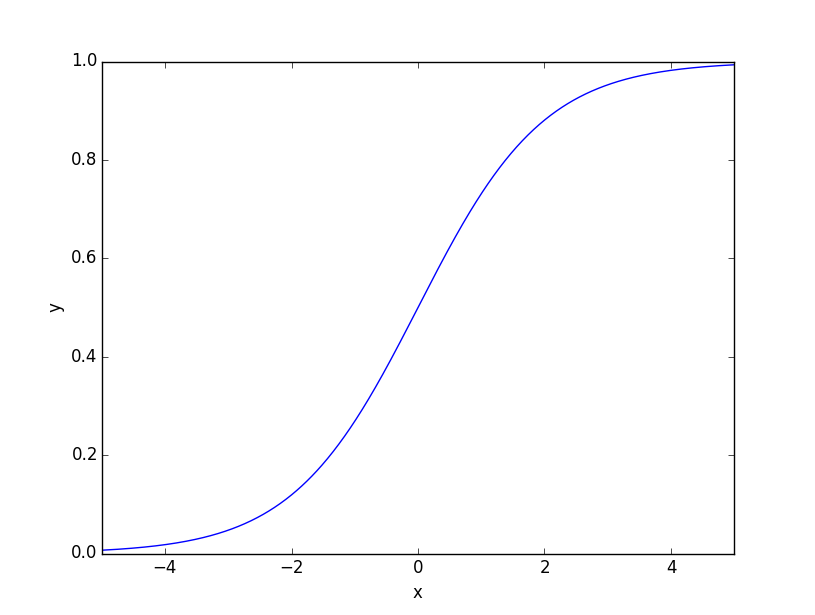
\includegraphics[width=0.4\linewidth]{./img/sigmoid.png}
	      \end{center}
	      \caption{Gráfico de la función Sigmoide}
	      \label{fig:sigmoid}
	    \end{figure}

	  \subsubsection {Tangente hiperbólica}
	    \begin{figure}[H]
	      \begin{center}
	       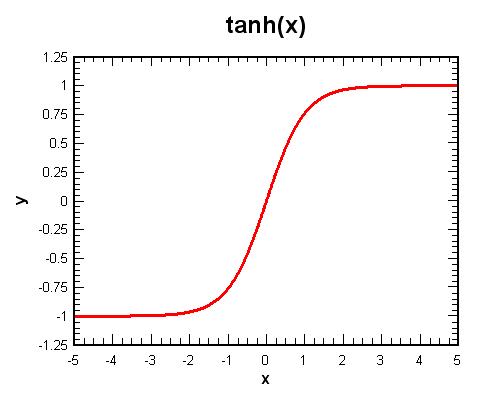
\includegraphics[width=0.4\linewidth]{./img/tanh.png}
	      \end{center}
	      \caption{Gráfico de la función Tangente hiperbólica}
	      \label{fig:tanh}
	    \end{figure}
	    Proyecta el dominio al rango [-1,1], como se muestra en la figura \ref{fig:tanh}. Al igual que la neurona sigmoide, sus activaciones saturan, pero a diferencia
	    de la neurona sigmoide su salida esta centrada en cero. Por lo tanto, en la práctica la tanh siempre es preferida sobre sigmoide.
	    \FIXME{CORREGIR}
	    \begin{equation*}
	     f(x) = max(0,x)
	    \end{equation*}

	  \subsubsection {ReLU}
	    La Unidad Rectificada Lineal (Rectified Linear Unit en la literatura en inglés) se ha vuelto muy popular en los últimos años. Toma el máximo entre el valor y cero, es decir
	    simplemente le agrega un umbral igual a 0, su gráfico se puede ver en la figura \ref{fig:relu}.
	    \begin{equation}
	     f(x) = max(0,x)
	    \end{equation}
	    \begin{figure}[H]
	      \begin{center}
	       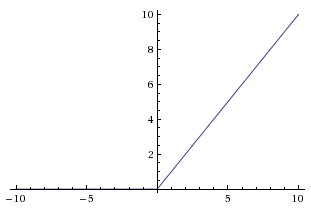
\includegraphics[width=0.4\linewidth]{./img/relu.jpeg}
	      \end{center}
	      \caption{Gráfico de la función ReLU}
	      \label{fig:relu}
	    \end{figure}

	    Las unidades lineales rectificadas son fáciles de optimizar porque son muy similares a las unidades lineales.
	    La única diferencia entre una unidad lineal y una unidad lineal rectificada es que una unidad lineal rectificada da salida a cero a través de la mitad de su dominio.
	    Esto hace que las derivadas a través de una unidad lineal rectificada permanezcan grandes siempre que la unidad esté activa.
	    Los gradientes no sólo son grandes sino también consistentes.\\
	    Algunas ventajas de utilizar ReLUs:
	    \begin{itemize}
	      \item Se encontró que aceleran en gran medida la convergencia del descenso del gradiente estocástico en comparación con las funciones sigmoides/tanh, esto se debe a su forma lineal, sin saturarse.
	      \item En comparación con las funciones tanh/sigmoide que implican operaciones caras, la ReLU puede implementarse simplemente marcando una matriz de activaciones a cero.
	    \end{itemize}

	    Existen varias generalizaciones de unidades lineales rectificadas. La mayoría de estas generalizaciones se comportan de forma comparable a las unidades lineales rectificadas
	    y, en ocasiones, tienen un mejor desempeño. Un inconveniente para las unidades lineales rectificadas es que no pueden aprender a través de métodos basados ​​en
	    gradiente en ejemplos para los cuales su activación es cero. Una variedad de generalizaciones de unidades lineales rectificadas garantizan que reciben gradiente en
	    todas partes. Existen generalizaciones sobre esta, que agregan un parámetro de regularización:
	    \begin{itemize}
	      \item Leaky ReLU: Agrega un parámetro de fuga $\alpha$, fijándolo en un valor pequeño como por ejemplo 0.01.
		\begin{equation}
		  f(x)=1(x<0)(\alpha x)+1(x>=0)(x)
		\end{equation}
	      \item ReLU Paramétrica: Trata el parámetro de fuga como un parámetro aprendible. \FIXME{AGREGAR FORMULA}
	    \end{itemize}

      \subsection {Regularización: Marginación}
	\FIXME{DESARROLLAR MAS, EXPLICAR COMO SE HACE, QUE EFECTO TIENE}
	La marginación (Dropout en la literatura en ingles) es una técnica de regularización para reducir la saturación en redes neuronales previniendo el sobreajuste.
	El término "marginación" se refiere a dejar de lado algunas unidades (ocultas y visibles) en una red neuronal, a la hora de entrenar la red.
	\begin{figure}[H]
	  \begin{center}
	   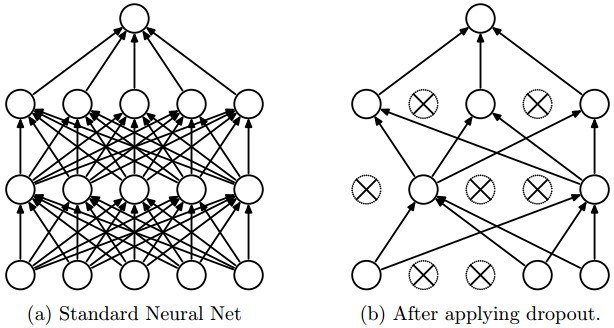
\includegraphics[width=0.6\linewidth]{./img/dropout.jpeg}
	  \end{center}
	  \caption{Durante el entrenamiento, la Marginación puede ser interpretada como tomar una subred Neuronal dentro de toda la Red Neuronal, y sólo actualizar los parámetros
	  de las subred basado en los datos de entrada. \cite{Srivastava:Dropout} }
	  \label{fig:dropout}
	\end{figure}

  \section {Aprendizaje Profundo}
    La caída de los precios de hardware y el desarrollo de GPUs para uso personal en los últimos años y la gran disponibilidad de datos, han contribuido al desarrollo del
    concepto de aprendizaje profundo (Deep Learning en ingles)
    que consiste de redes neuronales artificiales, que poseen mas de una capa oculta (se considera capa oculta a toda capa que no sea la de entrada ni salida). Este enfoque trata de
    modelar la forma en que el cerebro humano procesa luz y sonido en visión y audición.
    Algunas aplicaciones exitosas del aprendizaje profundo son la visión por computadora y el reconocimiento del habla.

    \subsection {Motivación}
      Los algoritmos simples de aprendizaje automático funcionan muy bien en una amplia variedad de problemas importantes.
      Sin embargo, no han logrado resolver los problemas centrales de Inteligencia Artificial, como reconocer el habla o reconocer objetos.
      El desafío de generalizar a nuevos ejemplos se vuelve más difícil cuando se trabaja con datos de gran dimensión y los mecanismos utilizados para lograr la generalización
      en el aprendizaje  automático tradicional son insuficientes para aprender funciones complicadas en espacios de alta dimensión.
      Tales espacios también suelen imponer altos costos computacionales. El aprendizaje profundo fue diseñado para superar estos y otros obstáculos.

  \section {Redes Neuronales Convolucionales}
    Las redes neuronales convolucionales (CNN) son muy similares a las redes neuronales antes vista, con la diferencia en que la arquitectura de una red neuronal convolucional asume explícitamente
    que el conjunto de entrada son imágenes, lo que le permite codificar ciertas propiedades dentro de la arquitectura.
    Están inspiradas en las redes neuronales tradicionales, incorporando operaciones no-lineales de manipulación de imágenes, suelen tener un gran numero de capas ocultas, por lo que
    son consideras parte del Aprendizaje Profundo.
    Con lo que respecta a las imágenes, muchos de los enfoques modernos en Visión por Computadoras explotan la propiedad de que píxeles cercanos están más correlacionados entre ellos que a los píxeles mas
    distantes, mediante la extracción de características locales que dependen sólo pequeñas subregiones de la imagen. La información de tales características pueden entonces ser combinados
    en etapas posteriores de procesamiento con el fin de detectar de características de alto nivel hasta finalmente proveer información de la imagen completa. Además, las características
    locales que son útiles en una región de la imagen, probablemente sean útiles en otras regiones de la imagen. \FIXME{BISHOP 285 }
    \subsection{Función de Convolución}
      \FIXME{Definir función de convolución}
      \FIXME{Hablar de filtro}
    \begin{figure}[H]
      \begin{center}
       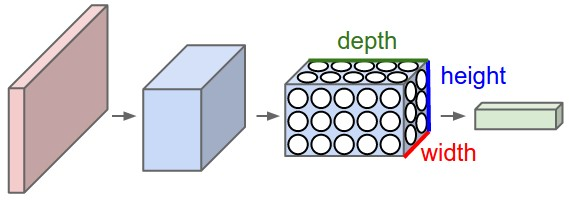
\includegraphics[width=0.8\linewidth]{./img/stanford_cnn.jpeg}
      \end{center}
      \caption{A la izquierda: Red Neuronal regular de 3 capas. A la derecha: Una CNN ordena a sus neuronas en tres dimensiones (ancho, alto, profundidad), como se visualiza en una de
	las capas. Cada capa de una CNN transforma un volumen 3D de entrada a un volumen 3D de salida. En este ejemplo, en la capa de entrada se encuentra la imagen, por lo que su ancho y su altura
	serían las dimensiones de la imagen, y la profundidad sería 3 (los canales Rojo, Verde, Azul). \cite{Karpathy:Stanford}}
      \label{fig:cnn}
    \end{figure}

    \subsection {Arquitectura de una red neuronal convolucional}
      En las redes neuronales convolucionales, las neuronas dentro de una capa se organizan en 3 dimensiones: alto, ancho y profundidad, como se ilustra en la figura \ref{fig:cnn}.
      Cada capa acepta un volumen de 3 dimensiones como entrada y lo transforma en un volumen de salida de 3 dimensiones a través de una función diferenciable.
      Algunas capas pueden tener o no parámetros, al igual que hiper-parámetros. La entrada y salida de cada una de estas capas son conjuntos de arreglos llamados “mapas de features”.
      En el caso mas simple de arquitectura, la red transforma el volumen de una imagen de entrada en un volumen de salida, conteniendo los puntajes de cada clase para el problema de clasificación.
      Típicamente, las CNNs suelen además organizarse por etapas, cada etapa consiste de una capa convolucional, una no lineal y una de agrupamiento.
      A continuación se detallan estos tipos de capas.

    \subsection {Tipos de Capas}
      \subsubsection{Capa Convolucional}
	Los parámetros consisten en un conjunto de filtros aprendibles. Cada filtro el pequeño espacialmente(alto y ancho) pero se extiende sobre toda la profundidad del volumen de entrada.
	Durante el paso hacia adelante, se desliza o convoluciona el filtro a través del alto y ancho del volumen de entrada y se computa el producto punto entre los valores del filtro y los valores
	del volumen de entrada. A medida que se va deslizando el filtro sobre el ancho y el alto del volumen de entrada, se va generando un mapa de activación de 2 dimensiones que contiene los
	valores de respuesta de ese filtro en cada posición espacial.\\
	Intuitivamente, la red aprenderá los filtros que se activan cuando ven algún tipo de característica visual como un borde de cierta orientación o una mancha de algún color en la
	primera capa, o eventualmente panal entero o patrones de rueda en las capas más altas de la red. Dado que tendremos un conjunto de filtros en cada capa Convolucional,
	y cada uno de ellos producirá un mapa de activación bidimensional separado, estos se apilaran a lo largo de la dimensión de profundidad para producir el volumen de salida.\\

	\emph{Retropropagación}: El paso hacia atrás para una operación de convolución (tanto para los datos como para los pesos) es también una convolución (pero con filtros espacialmente invertidos).
	\begin{figure}[H]
	  \begin{center}
	   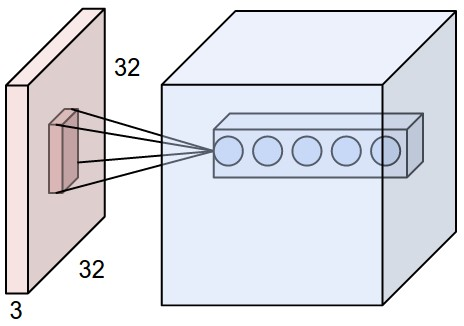
\includegraphics[width=0.8\linewidth]{./img/stanford_conv_layer.jpeg}
	  \end{center}
	  \caption{Un ejemplo del volumen de entrada (por ejemplo, un volumen de 32x32x3), y un ejemplo de volumen de neuronas en la primer capa Convolucional.
	    Cada neurona de la capa convolucional está conectada sólo a una región local en el volumen de entrada espacialmente, pero a la profundidad total (es decir, todos
	    los canales de color). Notar que hay múltiples neuronas (5 en este ejemplo) a lo largo de la profundidad, todos mirando en la misma región en la entrada.
	    A la derecha: Las neuronas de la Red Neuronal se mantienen sin cambios: Se calcula un producto punto de su peso con el de entrada seguido de una no-linealidad,
	    pero su conectividad está ahora restringida a ser local en el espacio. \cite{Karpathy:Stanford}}
	  \label{fig:conv_layer}
	\end{figure}

      \subsubsection{Capa de Agrupación}
	Su función es reducir progresivamente el tamaño espacial de la representación para reducir la cantidad de parámetros y de cálculo en la red, y por lo tanto también para controlar
	el sobreajuste. La capa de Agrupación (Pooling en la literatura en ingles) funciona independientemente en cada segmento de profundidad de la entrada y la redimensiona espacialmente, utilizando la operación de máximo,
	también se suele utilizar la operación de promedio o la norma L2.\\

	\emph{Retropropagación}: el paso hacia atrás para una operación máximo tiene una interpretación sencilla, ya que sólo encamina el gradiente a la entrada que tenía el valor más alto
	en el paso hacia adelante. Por lo tanto, durante el paso hacia adelante de una capa de agrupación es común realizar un seguimiento del índice de la activación máxima de
	manera que el enrutamiento de gradiente es eficiente durante la retropropagación.

	\begin{figure}[H]
	  \begin{center}
	   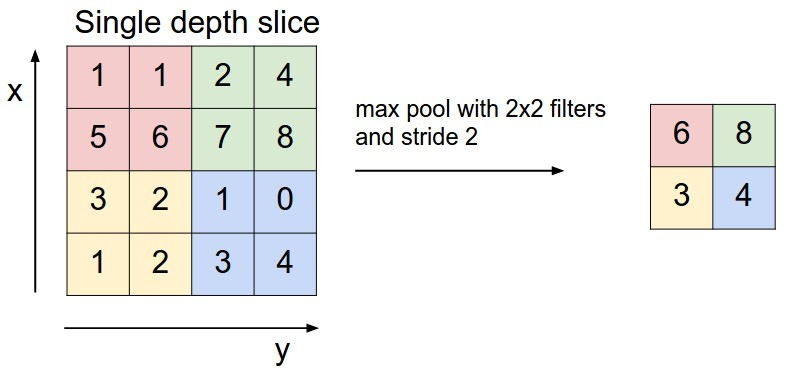
\includegraphics[width=0.8\linewidth]{./img/stanford_maxpool.jpeg}
	  \end{center}
	  \caption{La capa agrupación reduce el volumen espacialmente, de forma independiente en cada una profundidad de la entrada de volumen.
	    A la izquierda: En este ejemplo, el volumen de entrada de tamaño [224x224x64] es agrupado con un filtro de tamaño 2 y salto 2 en un volumen de salida de tamaño [112x112x64].
	    Observe que la profundidad del volumen se conserva. A la Derecha: la forma más común de reducción de tamaño de la operación de máximo, dando lugar agrupación por máximo,
	    que aquí se muestra, con un salto de 2. Es decir, cada operación se toma con 4 números (pequeño cuadrado de 2x2). \cite{Karpathy:Stanford}}
	  \label{fig:maxpool_layer}
	\end{figure}

      \subsubsection{Capas No Lineales}
	Estas capas son las encargadas de aplicar una función de activación no lineal, la principal funciones de activación utilizadas son las ReLU o alguna de sus variantes.

      \subsubsection{Capa Completamente Conectada}
	Las neuronas entre dos capas adyacentes están completamente conectadas de a pares, pero las neuronas dentro de una sola capa no comparten conexiones.

    \subsection {Consideraciones computacionales}
      El cuello de botella más grande a tener en cuenta al construir arquitecturas de CNN es la limitación de memoria.
      Muchas placas gráficas de procesamiento (GPUs en ingles) modernas tienen un límite de memoria de 3/4/6GB, las mejores GPUs que tienen cerca de 16GB de memoria.
      Hay tres fuentes principales de memoria para realizar un seguimiento:
      \begin{itemize}
	\item A partir de los tamaños de volumen intermedios: Éstos son el número crudo de activaciones en cada capa de la CNN, y también sus gradientes (de igual tamaño).
	  Normalmente, la mayoría de las activaciones se encuentran en las capas anteriores de una ConvNet (es decir, primeras capas de convolución).
	  Estos se mantienen ya que son necesarios para la retropropagación, pero una implementación inteligente que ejecuta una CNN sólo en la fase de prueba podría
	  en principio reducir esto en una cantidad enorme, sólo almacenando las activaciones actuales en cualquier capa y descartando las activaciones anteriores
	  en las capas de abajo.
	\item A partir de los tamaños de parámetro: Estos son los números que contienen los parámetros de red y sus gradientes durante la retropropagación.
	  Por lo tanto, la memoria para almacenar el vector de parámetros debe ser multiplicada por un factor de al menos 2 o más.
	\item Cada implementación de CNN tiene que mantener memoria datos extras, como los lotes de datos de imagen, tal vez sus versiones aumentadas, etc.
	\item Una vez que tenga una estimación aproximada del número total de valores (para activaciones, gradientes y extra). Si la red no entra en memoria, una heurística común
	  para que entre es disminuir el tamaño del lote, ya que la mayor parte de la memoria suele ser consumida por las activaciones.
      \end{itemize}


    \subsection {Casos de estudio de redes convolucionales famosas}

      \subsubsection{LeNet}
	 El primer éxito en las aplicaciones de Redes Neuronales Convolucionales, fue desarrollado por Yann LeCun en la década de 1990. La aplicación mas conocida que utiliza la arquitectura
	 LeNet es para leer los códigos postales, números, etc \cite{Lecun:LeNet}.

      \subsubsection{AlexNet}
	La primera obra que popularizó las Redes Neuronales Convolucionales en Visión por Computadoras fue el AlexNet, desarrollada por Alex Krizhevsky, Ilya Sutskever y Geoff Hinton.
	El AlexNet fue presentado al desafío ImageNet ILSVRC  en 2012 y obteniendo el primer puesto superando significativamente al segundo (top 5 de error de 16\% en comparación con el
	subcampeón con el 26\% de error). La Red tenía una muy arquitectura similar a LeNet, pero era más profundo, más grande, y capas convolucionales apiladas una encima de la otra
	(anteriormente era común tener solo capa convolucional siempre seguida inmediatamente por una capa de agrupación) \cite{AlexNet} .

      \subsubsection{GoogLeNet}
	El ganador de ILSVRC 2014 fue la Red Convolucional de Szegedy, proveniente de Google. Su contribución principal fue el desarrollo de un Módulo de "Inception" que reduce drásticamente
	el número de parámetros de la red (4M, en comparación con AlexNet con 60M). Además, en este documento se utiliza la agrupación por promedio en lugar de capas totalmente conectadas
	en la parte superior de la CNN, eliminando una gran cantidad de parámetros que no parecen influir mucho en el rendimiento \cite{Szegedy:Convolutions}.

      \subsubsection{VGG}
	El segundo puesto en ILSVRC 2014 fue la red de Karen Simonyan y Andrew Zisserman que llegó a ser conocido como VGG. Su contribución principal fue demostrar que la profundidad de
	la red es un componente crítico para el buen desempeño. Su version final contiene 16 capas convolucionales, que ofrece una arquitectura muy homogénea, sólo
	realiza convoluciones de 3x3 y agrupaciónes de 2x2 desde el principio hasta el final. Su modelo preentrenado está disponible para publicamente.
	Una desventaja de la VGG es que es más caro para evaluar y consume mucha más memoria y parámetros (140M). La mayoría de estos parámetros se encuentran en la primera
	capa totalmente conectada, y desde entonces se ha encontrado que estos capas pueden ser removidos con ningúna disminucion de rendimiento, reduciendo significativamente el
	número de parámetros necesarios \cite{SimonyanVGG} .

      \subsubsection{Resnet}
	Las Redes Residuales fueron desarrolladas por Kaiming He, que fue el ganador de ILSVRC 2015. La caracteristica particular de este tipo de redes es que  utilizan conexiones salteadas
	y hacen uso intensivo de la normalización por lotes.
	Esta arquitectura también solo tiene una capa completamente conectada en el extremo final de la red. ResNets actualmente son, por lejos, el estado del arte de las
	Redes Neuronales Convolucionales \cite{Kaiming:ResNet} .

    \section {Ajuste fino}
      %STANFORD
      El ajuste fino (Finetuning en inglés), es una tecnica que toma un modelo ya entrenado, con sus respectivos pesos,  y consiste en adaptar la arquitectura
      del modelo inicial, para el problema al cual se quiere emplear, brindando un conjunto de datos de entrenamiento con el cual se entrena la red adaptada,
      pero la inicializacion de los pesos coincide con los pesos obtenidos del modelo preentrenado.
      Por ejemplo una red fue entrenada para reconocer distintas razas de perros en imagenes, y ahora se desea clasificar gatos segun su raza. En lugar de entrenar una
      red desde un estado aleatorio inicial, se puede utilizar la red preentrenada para perros, reemplazando la ultima capa completamente conectada por otra que
      tenga la cantidad de salidas igual a la cantidad de razas de gato que se desean reconocer.
      Para el entrenamiento de esta red adaptada se le da como entrada un conjunto de imagenes, de gatos de las distintas razas, de esta forma los  pesos se van
      ajustando para lograr reconocer este nuevo tipo de conceptos en las imagenes.
      \FIXME{DESARROLLAR MEJOR EL EJEMPLO}
      \paragraph{Modelos preentrenados}
	Debido a que una red neuronal convolucional moderna requiere entre 2 y 3 semanas para entrenarse, utilizando multiples GPUs para el conjunto de datos ImageNet \cite{imagenet_cvpr09},
	es comun ver que gente publica sus Redes ya entrenadas para el beneficio de otras personas que lo pueden usar para hacer reentrandas, lo que requiere un tiempo mucho menor.

      \paragraph{Como y cuando hacer Reentrenamiento}
      \FIXME{REVISAR SI HACE FALTA PONERLO}
	¿Cómo decidir qué tipo de transferencia de aprendizaje debe realizar en un nuevo conjunto de datos? Esta es una función de varios factores, pero los dos más importantes son el
	tamaño del nuevo conjunto de datos (pequeño o grande), y su similitud con el conjunto de datos original (por ejemplo ImageNet-como en términos de contenido de imágenes y las clases,
	O muy diferentes, tales como imágenes de microscopio). Teniendo en cuenta que las características de CNN son más genéricas en capas tempranas y más específicas del conjunto de datos
	originales en capas posteriores, aquí hay algunas reglas comunes para navegar por los 4 escenarios principales:
	\begin{itemize}
	  \item El nuevo conjunto de datos es pequeño y similar al conjunto de datos original. Dado que los datos son pequeños, no es una buena idea afinar la red convolucional debido a las
	  preocupaciones excesivas. Dado que los datos son similares a los datos originales, esperamos que las características de mayor nivel en la red convolucional sean relevantes para este
	  conjunto de datos. Por lo tanto, la mejor idea podría ser la de formar un clasificador lineal utilizando las caracteristicas extraidas en la ultima capa de la red.
	  \item El nuevo conjunto de datos es grande y similar al conjunto de datos original. Dado que tenemos más datos, podemos tener más confianza de que no superaremos si intentáramos
	  ajustar a través de la red completa.
	  \item El nuevo conjunto de datos es pequeño pero muy diferente del conjunto de datos original. Dado que los datos son pequeños, lo más probable es que sólo entrenen un clasificador
	  lineal. Dado que el conjunto de datos es muy diferente, puede que no sea mejor entrenar al clasificador en la parte superior de la red, que contiene más características específicas
	  de conjunto de datos. En su lugar, podría funciónar mejor para entrenar el clasificador SVM de las activaciones en algún lugar anterior en la red.
	  \item El nuevo conjunto de datos es grande y muy diferente del conjunto de datos original. Dado que el conjunto de datos es muy grande, podemos esperar que podamos permitirnos
	  entrenar a una red convolucional desde cero. Sin embargo, en la práctica es muy a menudo todavía beneficioso para inicializar con pesos de un modelo pre-entrenado.
	  En este caso, tendríamos suficientes datos y confianza para afinar a través de toda la red.
	\end{itemize}

\chapter{Algoritmo de Transferencia de estilo}
    \section{Introducción}
      En este capitulo se desarrollan los contenidos específicos relativos al Algoritmo de Transferencia de Estilos artisticos a fotografías. El algoritmo elegido para tal fin es el que
      presenta Gatys et al. \cite{Gatys:Neural_Style}. \\
      En lo que al arte respecta, los humanos han desarrollado la capacidad de crear experiencias visuales únicas componiendo una compleja interacción entre el contenido y el estilo de una imagen.
      Sin ir mas lejos, las bases algoritmicas de este proceso se desconocen y no existen sistemas artificiales que con capacidades similares. Sin embargo, en otras areas fundamentales
      de la percepcion visual como el reconocimiento de objetos y rostros recientemente se ha alcanzado precisión cercana a la de un humano, utilizando modelos de redes neuronales profundas.
      Aquí se presenta un sistema artificial basado en una Red Neural Profunda que crea imágenes artísticas de alta calidad perceptiva. El sistema utiliza representaciones neuronales
      para separar y recombinar el contenido y el estilo de imágenes arbitrarias, proporcionando un algoritmo para la creación de imágenes artísticas.\\
      Inicialmente, el autor publica un articulo para sintetizar texturas naturales utilizando Redes Neuronales Convolucionales entrenadas para el reconocimiento de objetos,
      donde define a una textura como la correlación entre los distintos mapas de caracteristicas de cada una de las capas de la red \cite{Gatys:Texture_Synthesis}. Aplicando este enfoque
      logro obtener resultados muy interesantes como se muestran en la figura \ref{fig:textures}, en la parte inferior de la figura se muestra la imagen de muestra y en la parte superior
      se muestra la reconstrucción de la imagen a partir de los mapas de caracteristicas de una de las ultimas capas de la CNN. Ademas en la ultima columna se muestra la representación
      de una imagen que no corresponde a una textura, para dar una mejor intuicion de como se representa la informacion de la imagen.\\
      \textbf{Sintesis de texturas:}
      En el contexto del procesamiento de imagenes el concepto de textura hace referencia a imagenes digitales que se componen por elementos repetitivos a lo largo de la misma.
      La sintesis de texturas es el proceso de construir algoritmicamente una imagen digital de grandes dimensiones basandose en una muestra pequeña, respetando la estructura de su contenido. La Sintesis de
      texturas puede ser utilizada para rellenar agujeros en imágenes (como en los algoritmos de restauración) y la expansión de pequeñas imágenes.
      Los algoritmos de sintesis de texturas tienen como objetivo principal que la imagen generada sea lo mas parecida posible a la imagen de muestra que estan sintetizando.\\
      	\begin{figure}[H]
	  \begin{center}
	   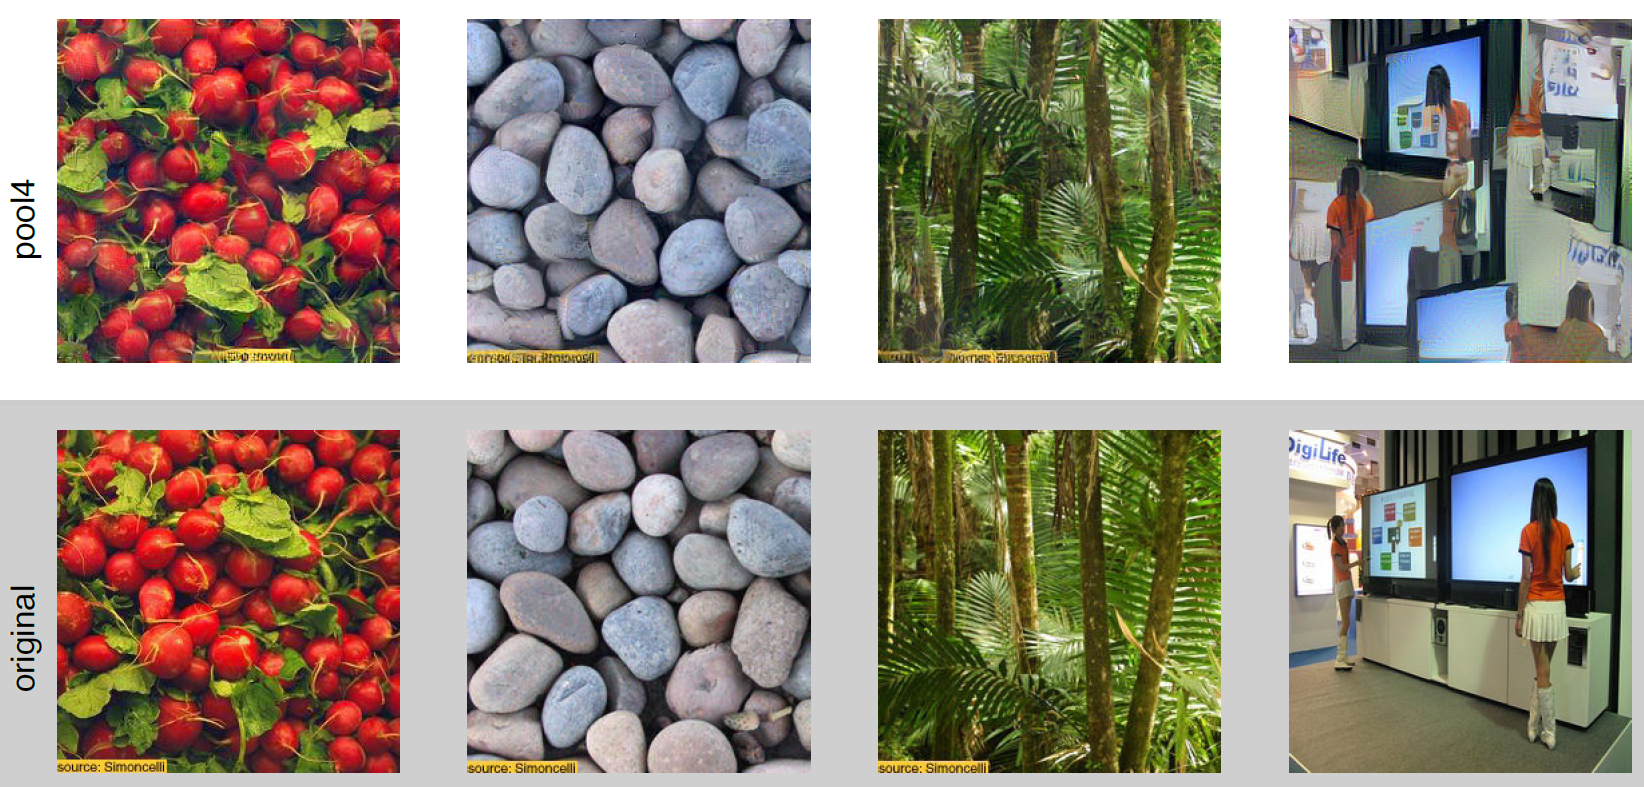
\includegraphics[width=0.8\linewidth]{./img/textures.png}
	  \end{center}
	  \caption{Ejemplos de sintesis de texturas utilizando Redes Neuronales Convolucionales}
	  \label{fig:textures}
	\end{figure}
      
    \section{Contexto}
      Transferir el estilo de una imagen a otra puede ser considerado un problema de transferencia de texturas. En la transferencia de texturas el objetivo es sintetizar la textura de la imagen
      de donde proviene, con algunas restricciones, de modo que permita preservar el contenido semantico de la imagen a la cual se le desea transferir la textura.
      Teniendo en cuenta todo esto, el autor adapta su idea propuesta para sintetizar texturas a la Transferencia de Estilos, problema que normalmente se encaraba en una rama de la visión de computadoras llamada representación
      no fotorrealista \cite{Kyprianidis:ArtisticStylization}. 
      Existen otros algoritmos que utilizan este enfoque de considerarlo como un problema de transferencia de texturas, por ejemplo: Hertzmann analogias de imagenes para transferir la 
      textura de una imagen de estilo a otra imagen \cite{Hertzmann:ImageAnalogies}, Ashkimin se centra en la transferencia de la informacion de alta frecuencia de la textura, 
      preservando la informacion a gruesa escala de la de la imagen de destino \cite{Ashikhmin:FastTextureTransfer}, Efros y Freeman introduce un mapa de correspondencias
      que incluye las características de la imagen de destino, tales como la intensidad de la imagen para restringir el proceso de sintetizacion de la textura \cite{Efros:ImageQuilting}, 
      Lee et al. mejora este algoritmo agregando a la tranferencia de textura, informacion adicional acerca de los contornos y bordes \cite{Lee:DirectionalTextureTransfer}.
      Aunque estos algoritmos logran resultados notables, todos ellos sufren de la misma limitación fundamental: usan sólo características de bajo nivel de la imagen de destino para 
      informar a la transferencia de textura. Idealmente, sin embargo, un algortimo de transferencia de estilo debe ser capaz de extraer la semántica del contenido de la imagen de 
      destino (por ejemplo, los objetos y el paisaje general) y, luego, informar al procedimiento de transferencia de textura para represente el contenido semántico de la imagen de destino 
      junto con el estilo de la imagen de origen. Por lo tanto, un requisito fundamental es encontrar representaciones de la imagen que, modelen independientemente las variaciones 
      de la semántica del contenido de la imagen y el estilo que se les presentan. Esto se puede lograr utilizando los mapas de caracteristicas de las Redes Neuronales Convolucionales 
      entrenadas en el reconocimiento de objetos, ya que se ha probado que estas logran extraer información semantica de alto nivel del contenido de las imagenes \cite{AlexNet}. \\
      La publicación de estos artículos, ha incentivado a muchos investigadores del area a continuar desarrollando estas ideas, a tal punto que hasta el dia de hoy se siguen publicando
      avances el tema, a gran velocidad.

    \section{Sintesis \label{sec:sintesis}}
      El algoritmo desarrollado conceptualmente es un algoritmo de tranferencia de texturas que restringe el metodo de sintetizacion de texturas utilizando mapas de caracteristicas
      de redes neuronales convolucionales. Dado que la modelizacion de la textura se basa en estas mismas representaciones, el metodo de transferencia de estilo se reduce a un problema
      de optimizacion en una unica red neuronal. Las imagenes son generadas minimizando la distancia entre los mapas de caracteristicas de las imagenes de entrada con los mapas de
      caracteristica de la imagen de salida.
      Cuando las Redes Neuronales Convolucionales (CNNs) son entrenadas para reconocimiento de objetos, desarrollan una representación de la imagen que hace que la información
      del objeto sea cada vez más explícita a lo largo de la jerarquia de las capas de la red. Por lo tanto, a lo largo de las distintas capas de la red,
      la imagen de entrada se transforma en representaciones que cada vez más se preocupan por el contenido real de la imagen en lugar del valor de sus píxeles.
      Podemos visualizar directamente la información que cada capa contiene sobre la imagen de entrada, reconstruyendo la imagen solo a partir de los mapas de caracteristicas
      de esa capa. Las capas más altas de la red capturan el contenido de alto nivel en términos de objetos y su ordenamiento en la imagen pero no se limitan a los valores de cada
      pixel. En  cambio, las reconstrucciones de las capas inferiores simplemente pretenden reproducir los valores exactos de píxeles de la imagen original y algunas formas
      basicas como lineas o curvas. Por lo tanto, tomaremos a los mapas de características en las capas superiores de la red como el contenido representado.
      Para obtener la representacion del estilo de la imagen de entrada, se usa un espacio de caracteristicas originalmente diseñado para capturar información de texturas.
      Este espacio de caracteristicas esta construido sobre las respuestas de los filtros de cada capa de la red. Consiste en la correlación entre las diferentes respuestas de los filtros.
      Incluyendo las correlaciones de multiples capas, se obtiene una representacion que captura información de la textura pero no del ordenamiento global de la imagen.
      Al reconstruir las imágenes a partir de las representaciones obtenidas, se puede observar que producen una version texturizada de la imagen que captura su
      apariencia general en terminos de colores y estructuras localizadas, a estas representaciones las llamaremos representaciones de estilo.
      El principal descubrimiento de este articulo es que la representacion del estilo y el contenido de una imagen pueden ser separables con una Red Neuronal Convolucional entrenada
      para el reconocimiento de objetos. De esta forma, al manipularse independientemente se pueden generar una nueva imagen desde 2 imágenes de entradas distintas, simultaneamente se corresponda con la representacion
      del contenido de una imagen y la respresentacion del estilo de la otra.\\
      Por otro lado el algoritmo presentado, requiere la definición de algunos hiperparametros, que afectan en gran medida al resultado generado.
      Al ser un problema de optimización, el numero de iteraciones en que se aplica el descenso por el gradiente determina cuanto se minimiza la funcion de perdida
      y por lo tanto que tanto se acerca la imagen generada al estilo de la imagen de estilo y el contenido a la imagen de contenido.
      Otros hiperparametros que requiere el algoritmo son definir cual sera la Red Convolucional utilizada y cuales seran las capas de la red empleadas para calcular el estilo y cual sera la capa elegida
      para calcular el contenido.
      	  \begin{figure}[h]
	    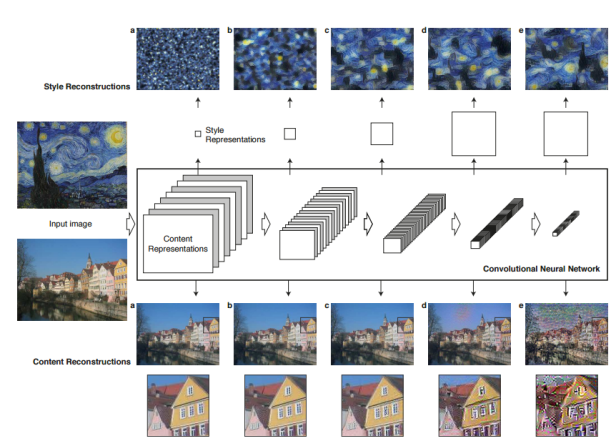
\includegraphics[width=\textwidth]{./img/gatys_1.png}
	    \caption{Reconstrucciones del Estilo y Contenido utilizando una CNN}
	    \label{fig:gatys_reconstrucciones}
	  \end{figure}
      En la figura \ref{fig:gatys_reconstrucciones} se pueden observar el resultado de reconstruir el estilo y el contenido utilizando los mapas de caracteristicas que se obtienen al
      realizar una pasada hacia adelante en la red VGG. Dada una imagen de entrada, en cada capa de la red, ésta se representa como el mapa de caracteristicas en respuesta a los filtros
      que pertenecen a esa capa. Mientras que el número de filtros va aumentando a lo largo de la jerarquía de la red, el tamaño de las representaciones de la imágenes va siendo reducido p
      or algunos mecanismos disminución de resolución(por ejemplo, agrupación) que conduce a una disminución en el número total de unidades por cada capa de la red.\\
      \textbf{Reconstruccion del contenido:}
	En la parte inferior de la figura \ref{fig:gatys_reconstrucciones} podemos visualizar la información en diferentes etapas de procesamiento en la CNN por la reconstrucción 
	de la imagen de entrada solamente conociendo las respuestas de los filtros 
	en una capa en particular. Al reconstruir la imagen de entrada a partir de las capas 'conv1\_1'(a), 'conv2\_1' (b), 'conv3\_1' (c), 'conv4\_1' (d) y 'conv5\_1' (e) de la red VGG,  
	se puede observar que la reconstrucción de las capas inferiores es casi perfecta (a,b,c). En cambio, en las capas más altas de la red, información detallada de los píxeles se 
	pierde, mientras que el contenido de alto nivel  de la la imagen se conserva (d,e). \\
      \textbf{Reconstruccion del estilo}:
	En la parte superior de la figura \ref{fig:gatys_reconstrucciones} construimos un nuevo espacio de características que captura el estilo de una imagen de entrada. 
	La representación de estilo se obtiene calculando las correlaciones entre los mapas de características de diferentes capas de la CNN. Al reconstruir el estilo de la imagen de estilo  
	utlizando diferentes subconjuntos de capas de la red ('conv1\_1' (a), "conv1\_1' y 'conv2\_1' (b), 'conv1\_1', 'conv2\_1' y 'conv3\_1' (c),'conv1\_1', 'conv2\_1', 'conv3\_1 ' y 'conv4\_1' (d), 
	'conv1\_1', 'conv2\_1', 'conv3\_1', 'conv4\_1' y 'conv5\_1' (e)). 
	Esto crea imágenes que coinciden con el estilo de la imagen dada, descartando la información del orden espacial de la escena.

    \section{Métodos \label{sec:metodos}}
      Los resultados exhibidos fueron obtenidos utilizando la red VGG-19, de disponibilidad publica \cite{SimonyanVGG}.
      Generalmente, cada capa de la red define un banco de filtros no lineal cuya complejidad aumenta con la posición de la capa en la red.
      Para visualizar la información de la imagen codificada en diferentes capas de la jerarquía se realiza descenso gradiente en una imagen de ruido blanco
      para encontrar otra imagen que coincida con las características de respuesta de la imagen original.
      Sea $\overrightarrow{x}$ la imagen de entrada, la cual será codificada por cada una de las capas de la red convolucional en un mapa de caracteristicas, basado en las respuestas de los filtros.
      Una capa con $N_l$ filtros distintos, tiene $N_l$ mapas de caracteristicas, cada uno de tamaño $M_l$, donde $M_l$ es el ancho por el largo del mapa de caracteristicas.
      Por lo tanto las respuestas de una capa $l$ pueden ser alojadas en una matriz $F^l \in R^{N_l \times M_l}$, donde $F_{i,j}^l$ es la respuesta del $i$-esimo filtro en la posición $j$.
      Entonces sean $\overrightarrow{p}$ y $\overrightarrow{x}$ la imagen original y la imagen generada, y sean $P^l$ y $F^l$ las respectivas representaciones en la capa $l$.
      Funcion Pérdida del Contenido se define como:
      \begin{equation}
       L_{contenido}(\overrightarrow{p},\overrightarrow{x}, l) = \frac{1}{2} \sum_{i,j} (F_{i,j}^l - P_{i,j}^l)^2
      \end{equation}
      El gradiente con respecto a la imagen $\overrightarrow{x}$ puede ser fácilmente calculado utilizando la retropropagación.
      Sobre las respuestas de la CNN en cada capa de la red construimos una representación de estilo que calcula las correlaciones entre las diferentes respuestas de los filtros.
      Estas correlaciones de las caracteristicas estan dadas por la matriz de Gram $G^l \in R^{N_l \times N_l}$, donde $G_{i,j}^l$ se calcula como el producto punto entre los vectores
      de los mapas de caracteristicas $i$ y $j$ en la capa $l$:
      \begin{equation}
	G_{i,j}^l = \sum_{k} F_{i,k}^l F_{j,k}^l
      \end{equation}

      Para generar una textura que coincida con el estilo de una imagen dada, utilizamos el descenso de gradiente de una imagen de ruido blanco para encontrar otra imagen que coincida
      con la representación de estilo de la imagen original. Esto se hace minimizando la distancia media cuadrada entre las entradas de la matriz de Gram de la imagen
      original y la matriz de Gram de la imagen a generar. Sean $\overrightarrow{a}$ y $\overrightarrow{x}$ la imagen original y la imagen generada, y sean $A^l$ y $G^l$
      las respectivas representaciones de estilo en la capa $l$, la contribución de esa capa a la función de perdida total del estilo es:
      \begin{equation}
       E_l = \frac{1}{4 N_l^2 M_l^2} \sum_{i,j} (G_{i,j}^l - A_{i,j}^l)^2
      \end{equation}
      La función de Pérdida del Estilo total queda definida:
      \begin{equation}
       L_{estilo}(\overrightarrow{a},\overrightarrow{x}) = \sum_{l=0}^{L} w_l E_l
      \end{equation}
      donde $w_l$ son los factores de peso que tiene cada capa sobre el resultado final. Los gradientes de $E_l$ con respecto a las activaciones de las capas de la red puede ser fácilmente
      calculado utilizando la retropropagación del error.
      Para generar las imágenes que mezclan el contenido de una fotografía con el estilo de una obra de arte conjuntamente minimizamos la distancia de una imagen de ruido blanco
      de la representación de contenido de la fotografía en una capa de la red y la representación de estilo de la obra de arte en un número de capas de la CNN.
      Funcion de Pérdida total:
      \begin{equation}\label{eq:objetivo}
       L_{total}(\overrightarrow{p},\overrightarrow{a},\overrightarrow{x}) = \alpha L_{contenido}(\overrightarrow{p},\overrightarrow{x}) + \beta L_{estilo}(\overrightarrow{a},\overrightarrow{x})
      \end{equation}
      Esta funcion combina linealmente las funciones de perdida del contenido y el estilo, por lo que se conforma por 2 terminos principales, uno correspondiente a la funcion de perdida
      del contenido y otro correspondiente a la funcion de perdida del estilo, donde $\alpha$ y $\beta$ son los factores de peso para el contenido y el estilo respectivamente, 
      a la hora de combinarlos. Por lo tanto, la salida del algoritmo, a partir de lo enunciado en la ecuación \eqref{eq:objetivo}, sera el argumento $\overrightarrow{x}$
      que minimice la funcion de perdida total, como se puede observar en la ecuacion \eqref{eq:resultante}. Para una mejor comprensión, en la figura \ref{fig:gatys_generacion} 
      se exhibe graficamente como funciona el algoritmo.
      \begin{equation} \label{eq:resultante}
       \overrightarrow{x} = \arg\min_{\overrightarrow{x}} L_{total}(\overrightarrow{p},\overrightarrow{a},\overrightarrow{x})
      \end{equation}

      \begin{figure}[h]
	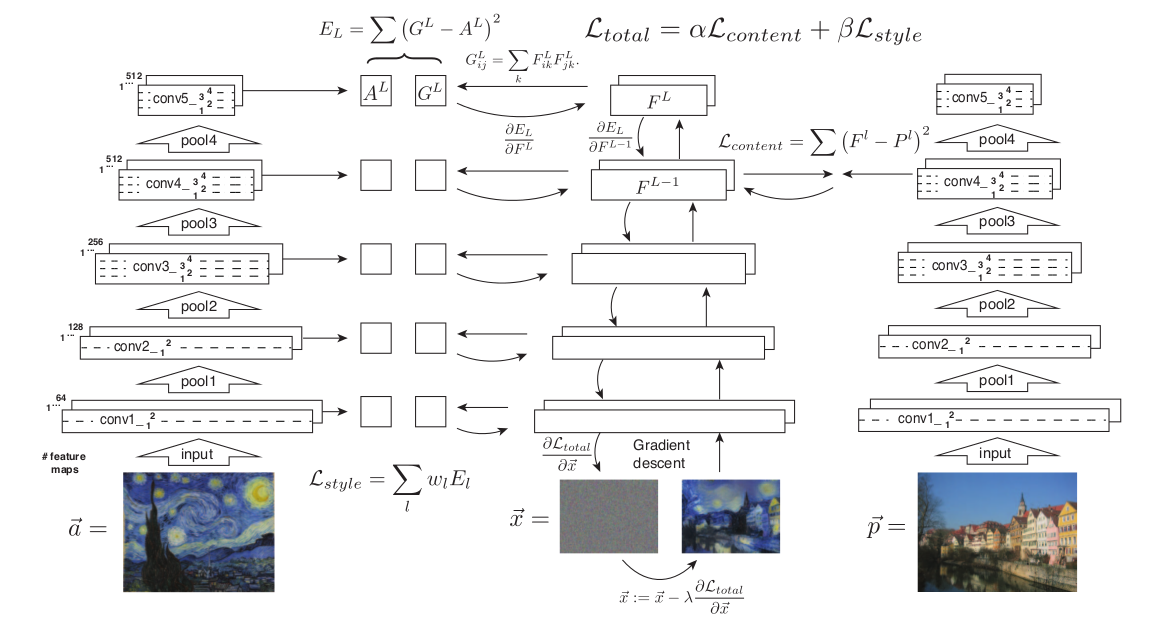
\includegraphics[width=\textwidth]{./img/gatys_method.png}
	\caption{Algoritmo de transferencia de estilo}
	\label{fig:gatys_generacion}
      \end{figure}
	A continuacion se realiza una explicacion detallada de lo que se muestra en la figura \ref{fig:gatys_generacion}: \\
	En primer lugar, las características de contenido y estilo se extraen y almacenan. La imagen de estilo $\overrightarrow{a}$ se pasa a través de la red
	y sus representaciones de estilo $A^l$ en todas las capas incluidas, son calculadas y almacenadas (a la izquierda). La imagen de contenido $\overrightarrow{p}$ pasa a través 
	de la red y la representación del contenido $P^l$ en una capa se almacena (a la derecha). Luego a partir de una imagen de ruido blanco $\overrightarrow{x}$ pasa a través de la red y sus
	características de estilo de $G^l$ y sus características de contenido $F^l$ son calculadas. \\
	En cada capa incluida en la representación de estilo, se calcula la diferencia cuadratica media punto a punto entre $G^l$ y $A^l$ para obtener la funcion de perdida del estilo
	$L_{estilo}$ (a la izquierda). Tambien se calcula la diferencia cuadratica media entre $F^l$ y $P^l$ para obtener la funcion de perdida del contenido $L_{contenido}$ (a la derecha).
	La función pérdida total $L_{total}$ es entonces una combinación lineal entre la función de perdida del contenido y la función de pérdida del estilo.
	La derivada de  $L_{total}$ con respecto a los valores de los píxeles pueden ser calculadas con el metodo  de retropropagación del error (en el medio). 
	Este gradiente se utiliza de forma iterativa actualizando la imagen $\overrightarrow{x}$ hasta que simultáneamente coincida con las características de estilo de la imagen 
	de estilo $\overrightarrow{a}$ y con las características de contenido de la imagen de contenido $\overrightarrow{p}$ (en la parte inferior central).


\chapter{Elección Automatica de hiperparámetros para Transferencia de estilo}
  \section{Descripción del problema}
    Basado en el algoritmo de transferencia de estilo se pueden obtener resultados muy interesantes, sin embargo, como se menciona en la sección \ref{sec:sintesis}
    es necesario definir el número de iteraciones como un hiperparámetro, que necesita el algoritmo para poder ejecutarse.
    El criterio de elección de este hiperparámetro termina siendo muy influyente en el resultado final. A medida que el número de iteraciones
    aumenta, la función de pérdida del resultado obtenido se va pareciendo cada vez a la función de pérdida calculada a partir de las imagenes de entrada, sin embargo,
    esto influye notablemente en el tiempo de ejecución requerido por el algoritmo.

    \subsection{Evaluación \label{sec:evaluacion}}
      Para poder realizar una comparación entre los distintos resultados generados por el algoritmo, es necesario establecer una métrica, que permita definir si un resultado
      obtenido es mejor que otro, debido a que en lo que respecta a las obras de arte, las evaluaciones suelen ser cualitativas en lugar de cuantitativas.
      Por ello es que se debe buscar una forma de cuantificar estos aspectos cualitativos.

  \section{Solución propuesta \label{sec:solucion}}
    En la solución propuesta en este trabajo se plantea poder definir automáticamente el número de iteraciones que debe ejecutarse el algoritmo hasta lograr obtener un resultado
    aceptable en la minima cantidad de iteraciones posible, reduciendo de esta forma el tiempo de ejecución del algoritmo.
    Con respecto al resto de los hiperparámetros  requeridos por el algoritmo, estos permanecen predefinidos de  antemano.
    La solución consta de 3 módulos principales: un módulo encargado de la generación de la imagen (a partir de una imagen de contenido y otra de estilo), otro módulo encargado de
    evaluar la imagen generada, y un tercer modulo que determina, en base al puntaje de clasificacion obtenido si es necesario continuar el proceso de generacion, como se puede
    observar en la figura \ref{fig:diagrama}.

    \begin{figure}[h]
      \begin{center}
	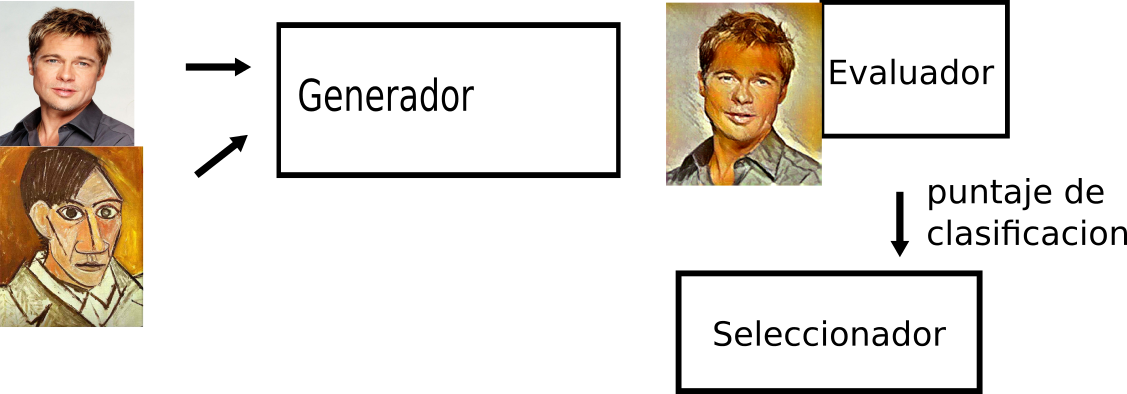
\includegraphics[width=\linewidth]{./img/diagrama.png}
      \end{center}
      \caption{Diagrama de interaccion entre los distintos modulos propuestos}
      \label{fig:diagrama}
    \end{figure}

    \subsection{Módulo de generación de imágenes \label{sec:generador}}
      En este modulo se implementa el algoritmo propuesto por Gatys, para la transferencia de estilo, que requiere como entrada una imagen de estilo,
      una imagen de contenido y como hiperparametro el numero de iteraciones que se ejecutara el optimizador para generar el resultado final.
      La salida de este es una imagen generada donde el contenido se acerca a la imagen de contenido y el estilo se acerca a la imagen de estilo, a medida
      que va aumentando el numero de iteraciones la distancia entre las imagenes de entrada y la imagen generada se va minimizando. Para mas detalles
      acerca del funcionamiento de este modulo, ver figura \ref{fig:gatys_generacion}.
    
    \subsection{Módulo de evaluación de imágenes: Reconocimiento de estilo \label{sec:evaluador}}
      Como se mencionó en Sec.~\ref{sec:evaluacion}, una de las limitaciones del proceso de transferencia de estilo es que la evaluación de
      la imagen resultante es de carácter cualitativo. A fin de establecer una medida cuantitativa y así controlar el resultado de la generación de
      manera más objetiva, se propone definir un clasificador, que se encargue de reconocer el estilo de una imagen, brindando un puntaje de clasificacion para cada estilo.
      De esta forma la imagen se evalua cuantitativamente segun el puntaje obtenido en el estilo objetivo.
      La entrada de este modulo es la imagen generada y la salida es los puntajes de clasificacion obtenidos por la imagen para cada uno de los estilos.\\

      A partir de la idea de definir un clasificador de estilos, se realizó una investigación de los posibles metodos para lograr esto. Se decidio basarse en el algortimo presentado en \cite{Karayev:Style_Recognition}.
      Este articulo plantea que los vectores de caracteristicas obtenidos de Redes Neuronales Convolucionales entrenadas para el reconocimiento de objetos, son muy utiles a la hora de
      reconocer estilos, aunque muchos estilos parecieran ser principalmente definidos por las elecciones de colores, los vectores de caracteristicas de las CNN, proveen mucha mas información
      que los vectores obtenidos a partir de histogramas de colores por ejemplo.
      Basado en esta idea, decidimos implementar una version simplificada que consiste en realizar ajuste fino sobre una Red Neuronal Convolucional preentrenda para el reconocimiento de objetos.
      De esta forma se van realizando evaluaciones de la imagen de salida obtenido por el algoritmo generador contra la predicción que realiza el modelo reentrenado para el reconocimiento de estilos.

    \subsection{Módulo de Selección \label{sec:seleccion}}
      Este modulo es el encargado de determinar si es necesario seguir generando imagenes o se acepta la imagen obtenida en la iteracion actual. La entrada de este modulo
      es el vector de puntajes de clasificacion calculados por el modulo generador \ref{sec:generador}, y la salida es un valor binario indicando si se acepta o no la imagen.
      El criterio de selección que se propone para elegir la imagen óptima es el siguiente:
      Basado en la hipotesis de que el resultado generado por el modulo generador \ref{sec:generador} obtenga un puntaje similar que la imagen de estilo en el modulo evaluador
      \ref{sec:evaluador}, se define una tolerancia del $\pm 20\%$ con respecto al puntaje obtenido por la imagen de estilo, en caso de que el resultado obtenga un puntaje que pertenezca
      a este rango, la imagen es aceptada como resultado final, en caso contrario el generador debe seguir iterando hasta obtener un resultado que cumpla con este requisito.


\chapter{Experimentos}
 En este capitulo se exponen los experimentos realizados basados en la solución propuesta en la seccion \ref{sec:solucion}, que permiten validar o rechazar las hipotesis planteadas.
 Para ello se realizaron 2 experimentos principales: El primero consiste en crear un modulo de reconocimiento de estilos artisticos realizando ajuste fino sobre una CNN preentrenada
 para el reconocimiento de objetos. En el segundo experimento se realiza el analisis empirico para la elección del numero de iteraciones mediante el criterio de selección planteado en la
 seccion \ref{sec:seleccion}.

\section{Reconocimiento de estilo}
  Para implementar el modulo de reconocimiento de estilo se decidio realizar ajuste fino sobre una red neuronal convolucional preentrenada para el reconocimiento de objetos.
  A lo largo de esta seccion se detallan las caracteristicas de la implementación de este modulo.
  \subsection{Conjunto de datos}
    El conjunto de datos utilizado para en este trabajo, se construyo a partir del conjunto de datos llamado WikiArt \url{https://www.wikiart.org/}.
    Este conjunto de datos proviene de un proyecto de disponibilidad publica que tiene como objetivo principal hacer accesible el mundo del arte a cualquier persona y en cualquier lugar.
    WikiArt cuenta con una 150.000 obras de arte, de 2.500 artistas. Estas obras se encuentran en museos, universidades y otros edificios civiles de más de 70 países. Aunque la mayoría de estas obras de arte no está en la vista pública.
    Para la implementación de la solución, se utilizo un subconjunto, tomando los 10 estilos que mayor cantidad de obras de arte disponen. A continuacion se enumeran los estilos contemplados:
    \begin{enumerate}
      \item Impresionismo  (14433 obras de arte disponibles)
      \item Realismo (13595 obras de arte disponibles)
      \item Romanticismo (10563 obras de arte disponibles)
      \item Expresionismo (9747 obras de arte disponibles)
      \item Post Impresionismo (7226 obras de arte disponibles)
      \item Surrealismo (6636 obras de arte disponibles)
      \item Modernismo (5969 obras de arte disponibles)
      \item Barroco (5156 obras de arte disponibles)
      \item Simbolismo (4689 obras de arte disponibles)
      \item Neo Clasisimo (3306 obras de arte disponibles)
    \end{enumerate}
      A modo de ejemplo, en la figura \ref{mosaico_estilos} se muestra una imagen correspondiente a cada uno de los estilos elegidos.
	\begin{figure}
	  \begin{center}
	  \def\tabularxcolumn#1{m{#1}}
	  \begin{tabularx}{\textwidth}{@{}cXX@{}}
	  %
	  \begin{tabular}{cc}
	    \subfloat[Modernismo]{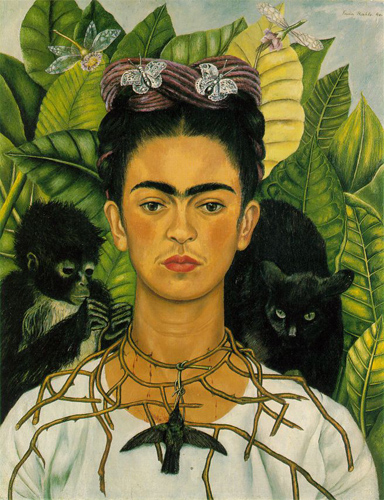
\includegraphics[height=0.15\textheight]{./img/frida_kahlo.jpg}}
	    & \subfloat[Impresionismo]{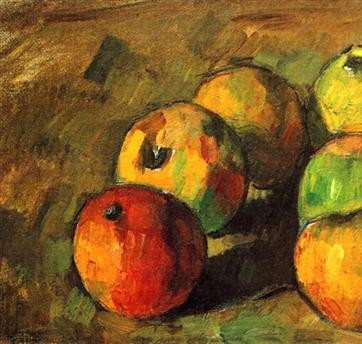
\includegraphics[height=0.15\textheight]{./img/cezanne.jpg}}\\
	    \subfloat[Surrealismo]{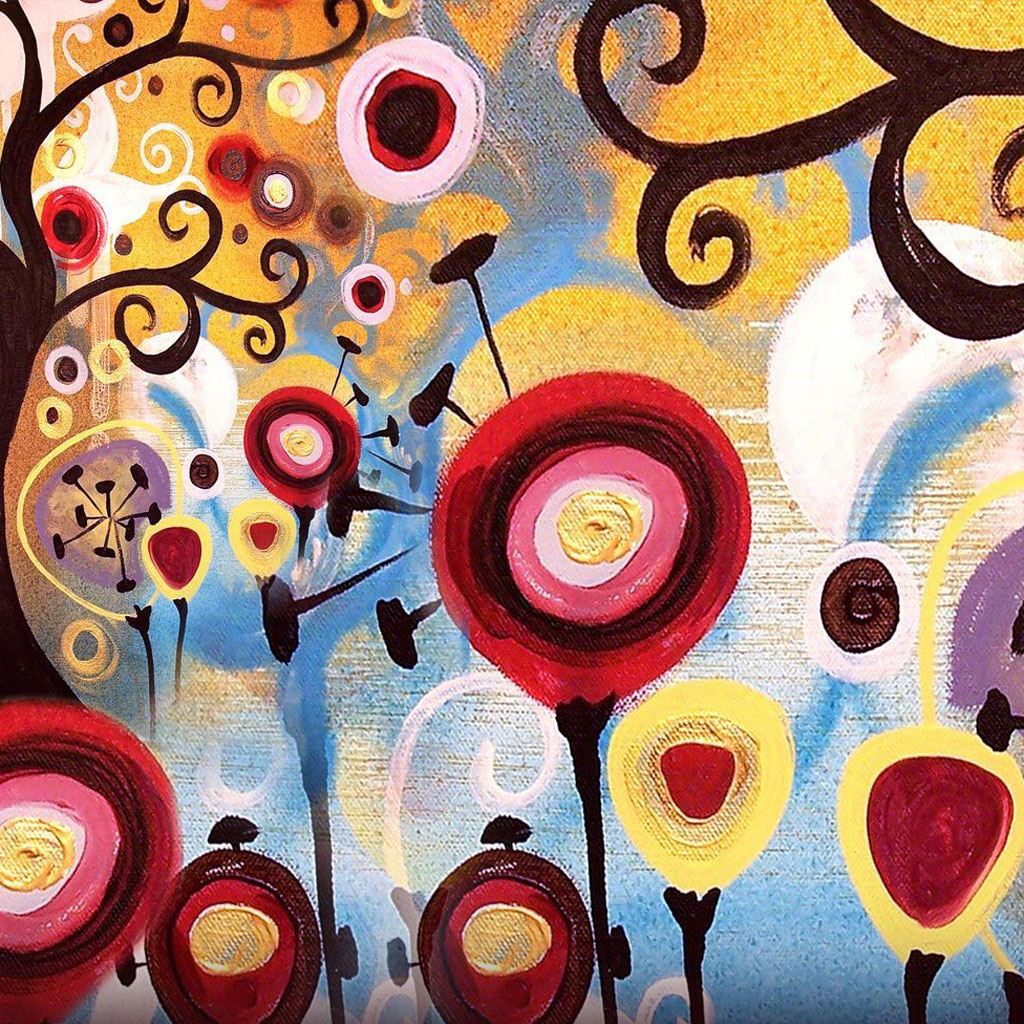
\includegraphics[ height=0.15\textheight]{./img/jhonson_style_candy.jpg}}
	    & \subfloat[Post Impresionismo]{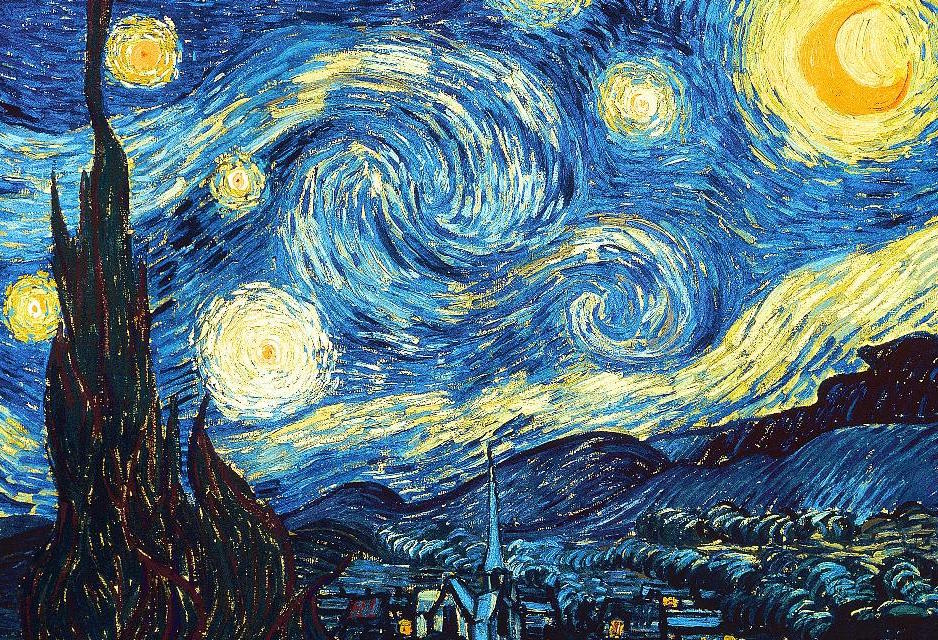
\includegraphics[height=0.15\textheight]{./img/starry_night.jpg}}\\
	    \subfloat[Simbolismo]{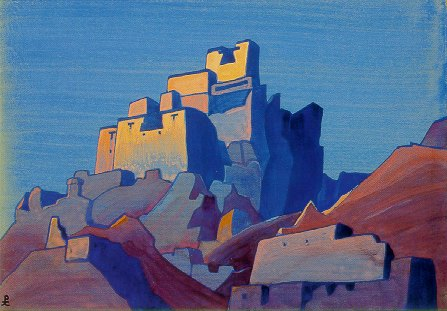
\includegraphics[ height=0.15\textheight]{./img/nicholas-roerich_chiktan-citadel-in-himalayas.jpg}}
	    & \subfloat[Neo Clasisimo]{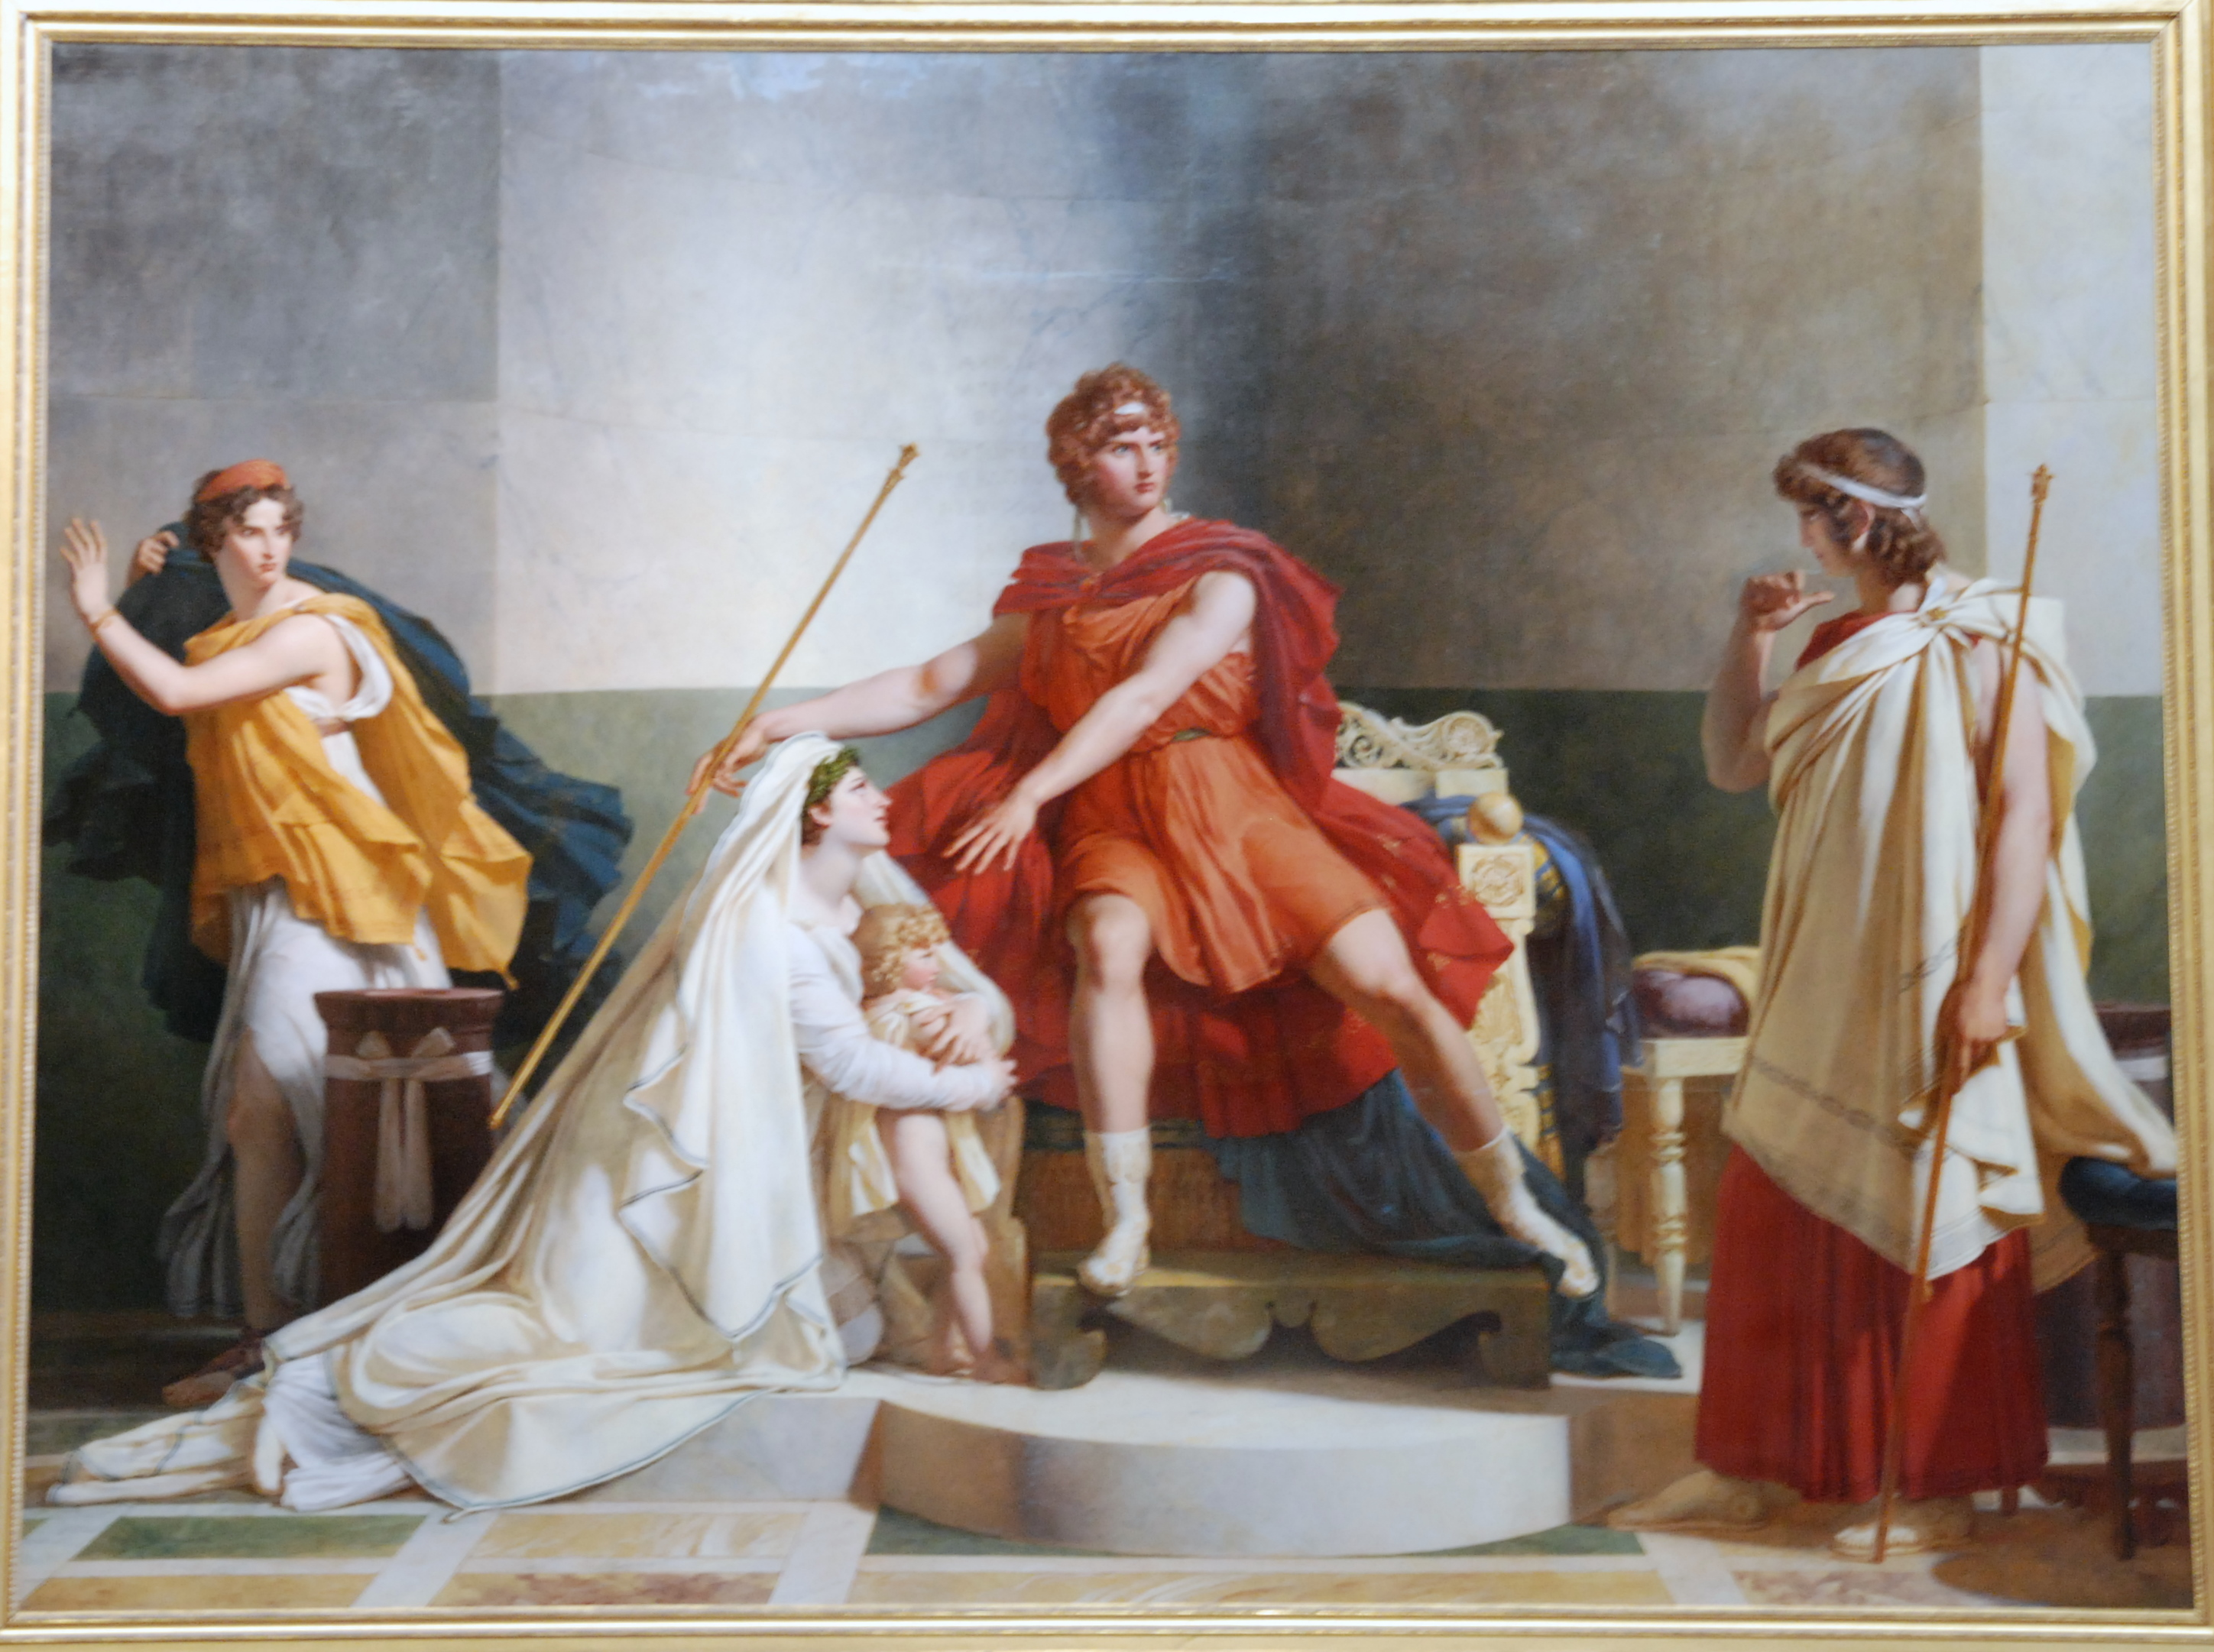
\includegraphics[height=0.15\textheight]{./img/pierre-narcisse-guerin_not-detected.jpg}}\\
	    \subfloat[Romanticismo]{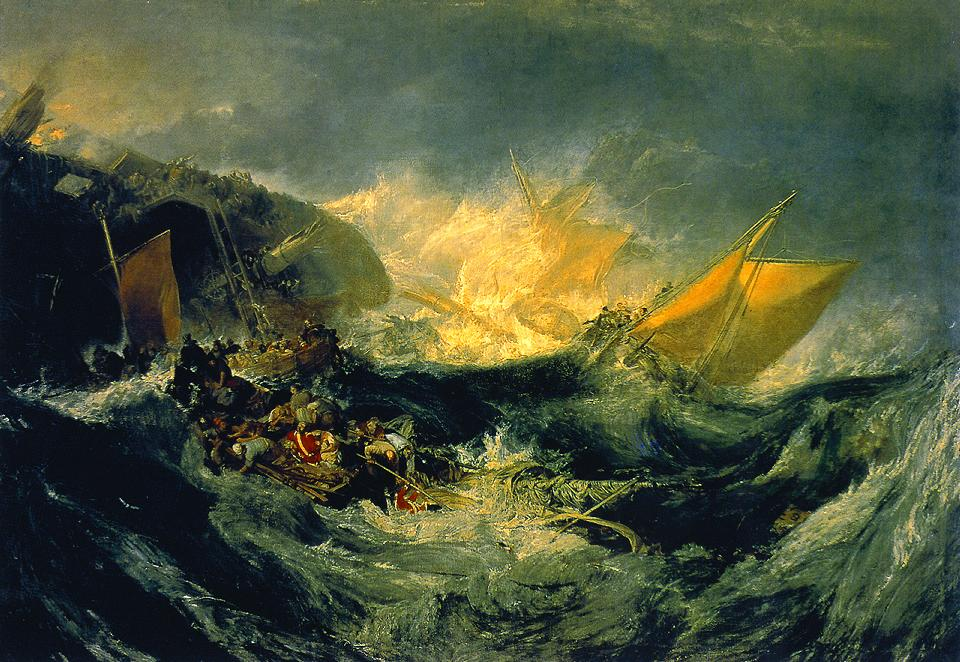
\includegraphics[height=0.15\textheight]{./img/shipwreck.jpg}}
	    & \subfloat[Barroco]{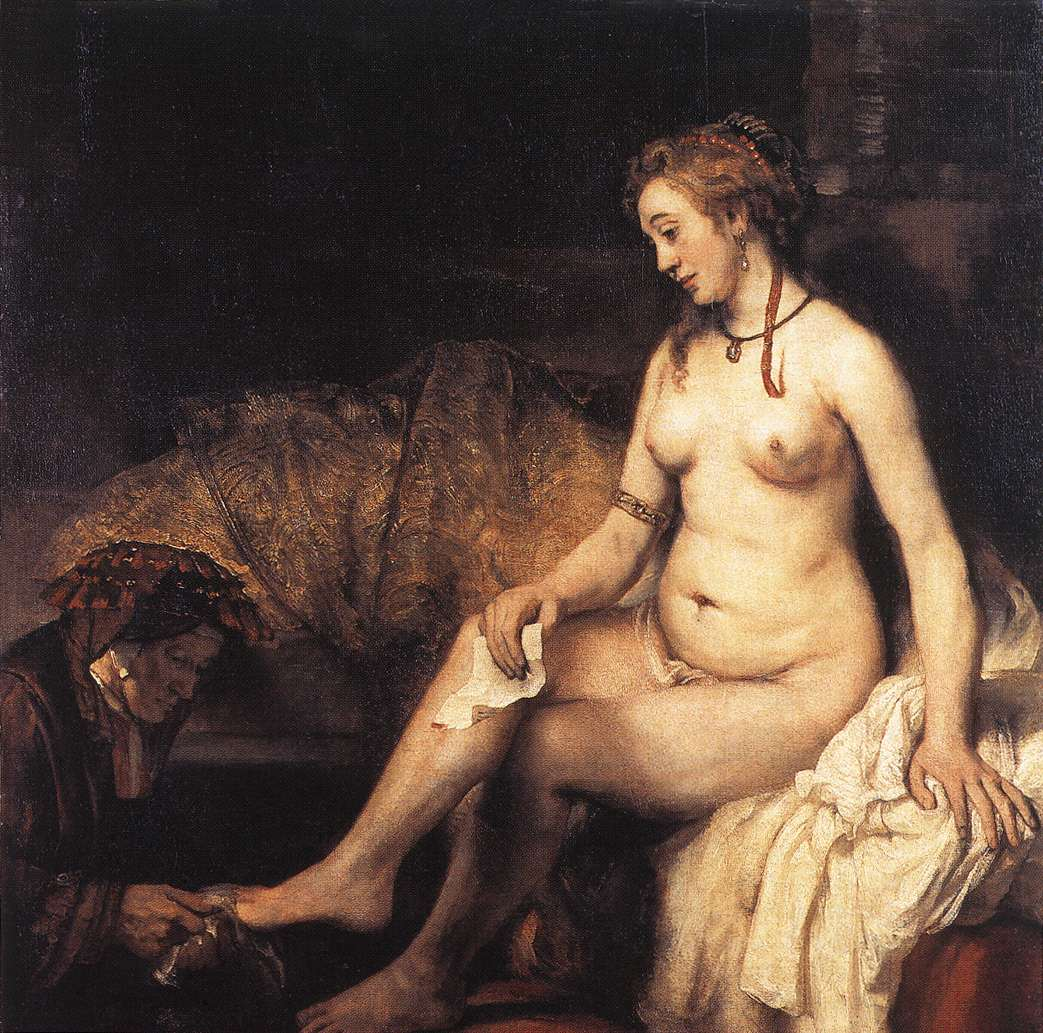
\includegraphics[height=0.15\textheight]{./img/rembrandt_bathsheba-bathing.jpg}}\\
	    \subfloat[Realismo]{\includegraphics[height=0.15\textheight]{./img/vincent-van-gogh_cart-with-red-and-white-ox.jpg}}
	    & \subfloat[Expresionismo]{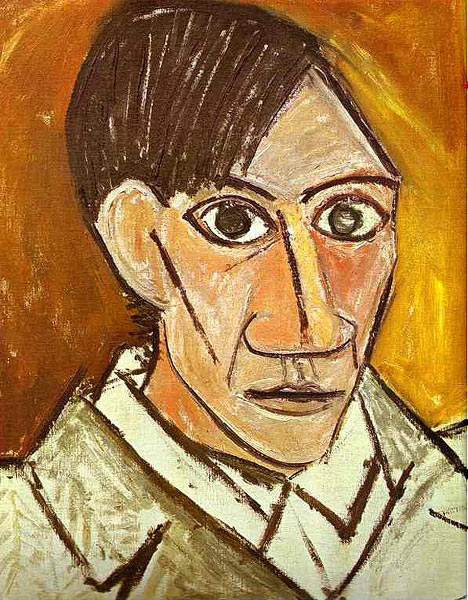
\includegraphics[height=0.15\textheight]{./img/picasso_selfport.jpg}}\\
	  \end{tabular}

	  \end{tabularx}

	  \caption{Ejemplos de obras de arte correspondientes a los estilos seleccionados}\label{mosaico_estilos}
	  \end{center}

	\end{figure}

      \subsubsection{Recolección y construcción del conjunto datos}
	El proceso de recoleccion y construccion de datos consistio en distintas etapas:
	\begin{enumerate}
	 \item Definir los 10 principales estilos de los que se dispongan mayor cantidad de obras, enumeradas anteriormente.
	 \item Descargar cada una de las obras de arte de todos los estilos seleccionados.
	 \item Verificar que la descarga haya sido exitosa y el archivo obtenido este en condiciones para ser utilizado en el proceso.
	 \item Ordenar los archivos segun el estilo al que pertenecen.
	 Luego de realizado este proceso, de las 81320 imagenes disponibles para los estilos elegidos, el conjunto de datos generado queda conformado por 68807 imagenes.
	\end{enumerate}

    \subsection{Detalles de implementación}
      Para realizar el ajuste fino, sobre este conjunto de datos generado, se utilizo la arquitectura de la red AlexNet \cite{AlexNet}, reemplazando la ultima capa por una capa que
      aprenda a reconocer entre los posibles estilos. Los valores con los que se inicializo la red, eran los valores obtenidos al entrenar AlexNet para el reconocimiento de objetos de ImageNet.
      Para reentrenar la red ajustando los valores para el reconocimiento de estilo, se le proveyo el conjunto de datos generado, y se definio realizar 50000 iteraciones para el ajuste fino.
      Para realizar el ajuste fino se utilizó las librerías Caffe y OpenCV en Python, y para el reentrenamiento fue requerido el uso de una GPU GTX 680.

    \subsection{Resultados de clasificación}
    La red obtuvo un 92 \% de precisión en el conjunto de entrenamiento al reconocer estilos.

  \section{Elección del número de iteraciones empleando el módulo de reconocimiento} 
    Este experimento consiste en realizar un analisis empirico de la evolucion de los puntajes de clasificacion de estilo a medida que aumenta el numero de iteraciones
    que se ejecuta el modulo de generacion de imagenes.
    \subsection{Conjunto de datos}
      Para ejecutar el procedimiento, es necesario disponer de 2 conjuntos de imagenes, uno correspondiente a las imagenes de contenido y otro correspondiente a las imagenes de estilo.
      Para el conjunto de imagenes de contenido fueron elegidas 5 imagenes, de las cuales 2 son retratos de personas y las 3 restantes son fotografias de paisajes.
      Con respecto al conjunto de imagenes de estilo, para cada uno de los estilos fueron elegidas 3 imagenes aleatoriamente.
    \subsection{Detalles de implementación}
      El proceso consistio en aplicar el algoritmo de transferencia de estilo combinando cada una de las fotos del conjunto de contenido con cada una de las fotos del conjunto de estilo,
      y guardando el resultado cada 10 iteraciones, hasta llegar a las 1000 iteraciones para cada uno de los procesos particulares.
      Ademas para cada combinacion de imagen de estilo e imagen de contenido el algoritmo se ejecuto 2 veces, una comenzando desde la imagen de contenido y otra comenzando desde una imagen de ruido.
      Finalmente todo el conjunto de imagenes obtenido es evaluado por el modulo de reconocimiento de estilo, que otorga un puntaje de la imagen para cada uno de los estilos.
      \subsubsection{Algoritmo de Transferencia de estilo}
	Existen una gran variedad de implementaciónes de código abierto que implementan el algoritmo de transferencia de estilo definido por Gatys.
	La que se decidió utilizar fue la de Justin Jhonson \cite{Johnson:Neural_Style}, la cual posee el mayor grado de aceptación en la industria.
	La principal tecnología utilizada en esta implementación es el Framework Torch, que utiliza como lenguaje de programación a Lua.
	La implementacion  utilizada, permite controlar algunas otras variables mediante hiperparametros extras a lo requerido por el algoritmo originalmente:
	Los principales hiperparámetros adicionales a los requeridos por el algoritmo son:
	\begin{itemize}
	  \item Modelo de Red Neuronal Convolucional preentrenada que se utilizará (existen una variedad de CNN presentadas anteriormente) junto con las capas que se utilizarán de la
	  respectiva red tanto para calcular el estilo como el contenido.
	  \item Imagen desde la cual comenzar la optimización, es posible comenzar desde una imagen de ruido, desde la imagen de contenido.
	  \item Método de optimización a utilizar.
	  \item Tamaño de la imagen generada
	  \item Peso de funciones de perdida de estilo y contenido en la funcion de perdida total \FIXME{esto lo requiere el algoritmo}
	  \item Tasa de aprendizaje para el optimizador
	\end{itemize}


    \subsection{Número de iteraciones vs. Puntaje de clasificación}
      Luego de generar distintas imagenes para cada uno de los estilos, variando entre imagenes de retratos y paisajes como imagenes de contenido, se realizó un analisis
      de la evolucion de los puntajes obtenidos por estas imagenes, a medida que el numero de iteraciones va aumentando. En esta seccion se presentan algunos casos de ejemplo
      que permiten ilustrar lo sucedido en la mayoria de los casos del conjunto de datos generado.\\
      El primer caso presentado en la figura \ref{fig:caso1_tubingen} es el mas simple, como imagen de estilo se utiliza The Shipwreck of the Minotaur, Joseph Mallord William Turner, 1805 (a),
      el cual pertenece al Romanticismo, y como imagen de contenido se utiliza una fotografia de un paisaje de la ciudad de Tubingen, Alemania (b).
      En la imagen (c) se puede observar el resultado obtenido partiendo desde una imagen de ruido, luego de 620 iteraciones y en la imagen (d) se puede observar el resultado partiendo desde 
      la imagen de contenido, luego de 600 iteraciones.
      La diferencia entre ambos resultados en este caso es sutil, pero al comenzar desde la imagen de contenido, los bordes y contornos de esta, son mas notorios en el resultado
      que al comenzar desde ruido.
        \begin{figure}[H]
	  \def\tabularxcolumn#1{m{#1}}
	  \begin{tabularx}{\textwidth}{@{}cXX@{}}
	  \begin{tabular}{cc}
	    \subfloat[Imagen de Estilo: Shipwreck, Turner, 1805]{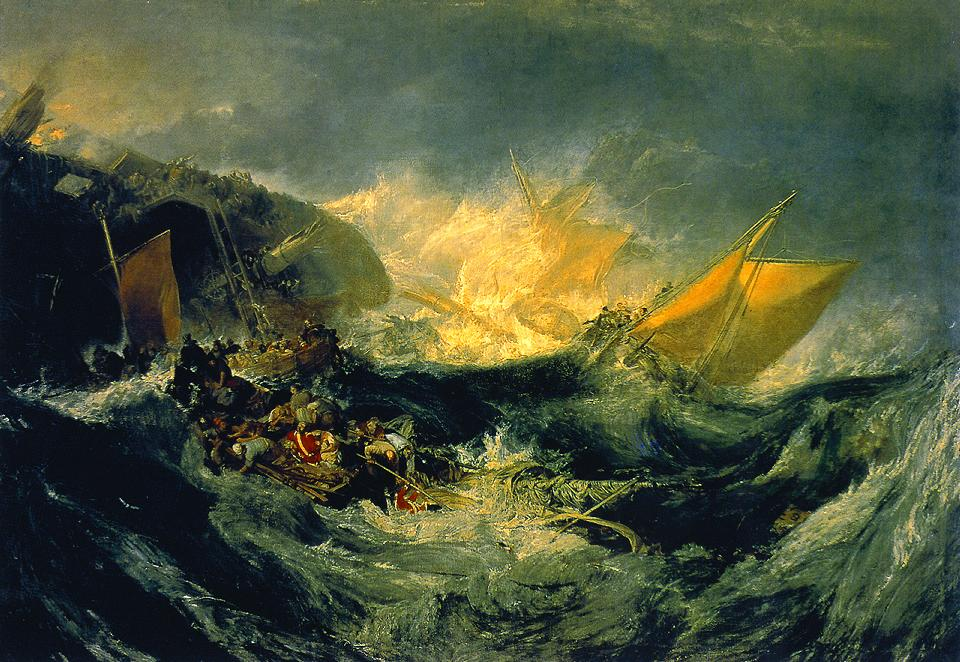
\includegraphics[height=0.2\textheight]{./img/shipwreck.jpg}}
	    & \subfloat[Imagen de Contenido: Fotografia de Tubingen]{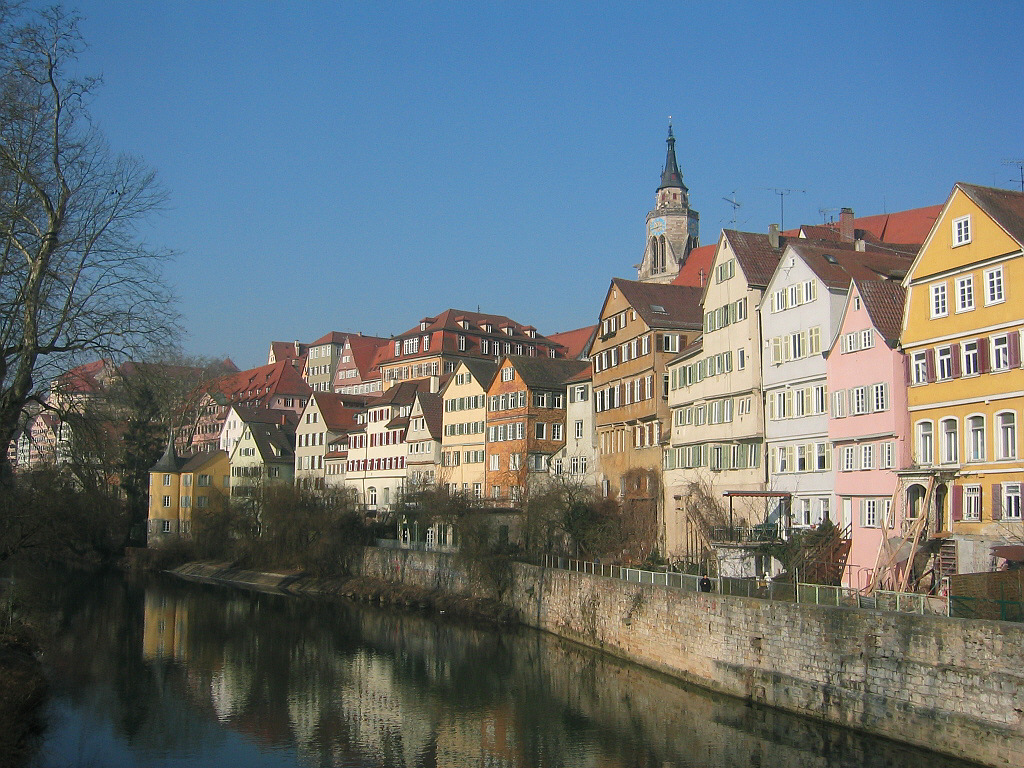
\includegraphics[height=0.2\textheight]{./img/tubingen.jpg}}\\
	    \subfloat[Resultado comenzando desde ruido]{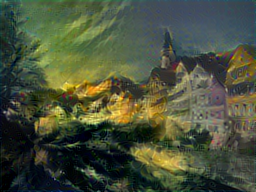
\includegraphics[ height=0.2\textheight]{./img/tubingen_shipwreck_620_random.png}}
	    & \subfloat[Resultado comenzando desde el contenido]{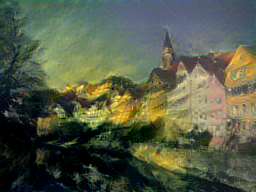
\includegraphics[height=0.2\textheight]{./img/tubingen_shipwreck_600_image.png}}\\
	  \end{tabular}
	  \end{tabularx}
	  
	  \caption{Ejemplos de obras de arte correspondientes a los estilos seleccionados}\label{fig:caso1_tubingen}
	\end{figure}
	En cuanto a la evolucion de los puntajes de clasificación, como se puede observar en la figura \ref{fig:puntajes_caso1}, en este caso se cumple con la hipotesis de que el 
	estilo predicho para el resultado coincide con el estilo de la imagen de estilo (Romanticismo), al partir desde una imagen de ruido, en las primeras 200 iteraciones el 
	clasificador no logra reconocer un claro estilo, pero luego se va normalizando hasta obtener una predicción confiable, ya que la diferencia con los otros estilos es notoria.
	\begin{figure}[H]
	  \begin{center}
	    \subfloat[Evolucion de los puntajes comenzando desde ruido]{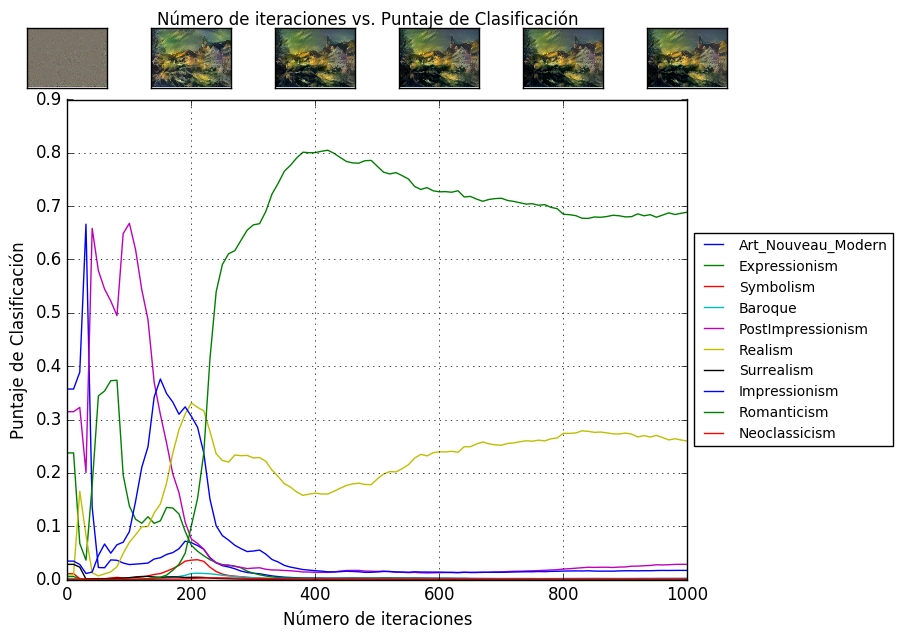
\includegraphics[ height=0.35\textheight]{./img/tubingen_shipwreck_random_scores.png}}\\
	    %\subfloat[Evolucion de los puntajes comenzando desde contenido]{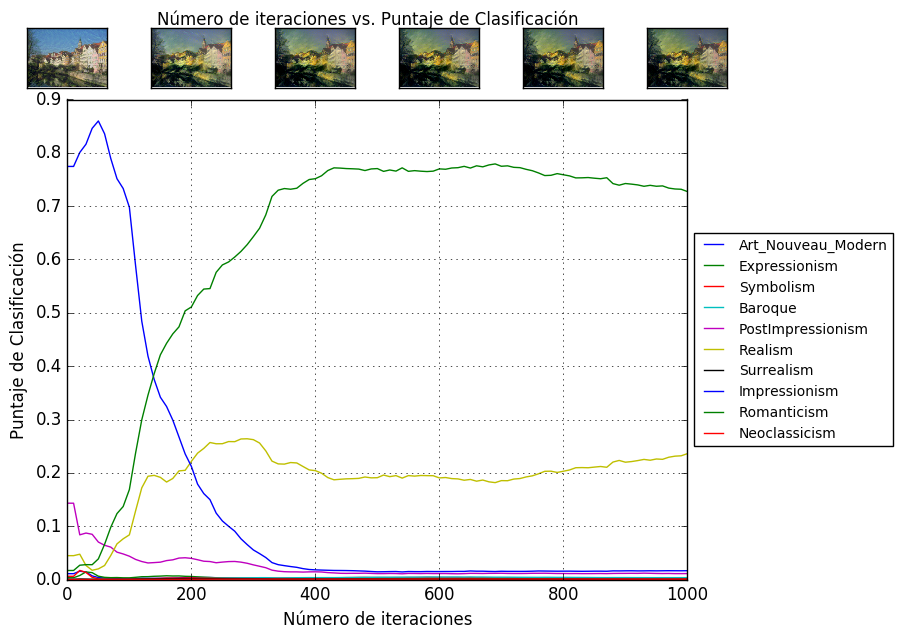
\includegraphics[height=0.4\textheight]{./img/tubingen_shipwreck_image_scores.png}}\\
	  \end{center}
	  \caption{Evolucion de los puntajes}
	  \label{fig:puntajes_caso1}
	\end{figure}
	
	Como segundo caso de analisis se eligio una situacion en la que la prediccion de la imagen resultante coincide con el estilo de la imagen de estilo provista, si se comienza
	el procedimiento desde la imagen de ruido, pero esto no ocurre si se comienza desde la imagen de contenido.
	Para este caso exhibido en la figura \ref{fig:caso2_scream}, como imagen de estilo se utilizo El grito, de Edward Munch, 1893 correspondiente al Expresionismo (a) y como imagen de contenido una fotografia del Golden Gate, un
	icono de la ciudad de San Francisco, Estados Unidos (b). En la imagen (c) se muestra el resultado partiendo desde ruido y en la (d) desde la imagen de contenido, ambas luego de
	540 iteraciones, desde el aspecto visual estos resultados son muy similares, pero para el clasificador son muy distintos como luego de muestra en la figura \ref{fig:puntajes_caso2}.
      
      	\begin{figure}[H]
	  \def\tabularxcolumn#1{m{#1}}
	  \begin{tabularx}{\textwidth}{@{}cXX@{}}
	  \begin{tabular}{cc}
	    \subfloat[Imagen de Estilo: The Scream]{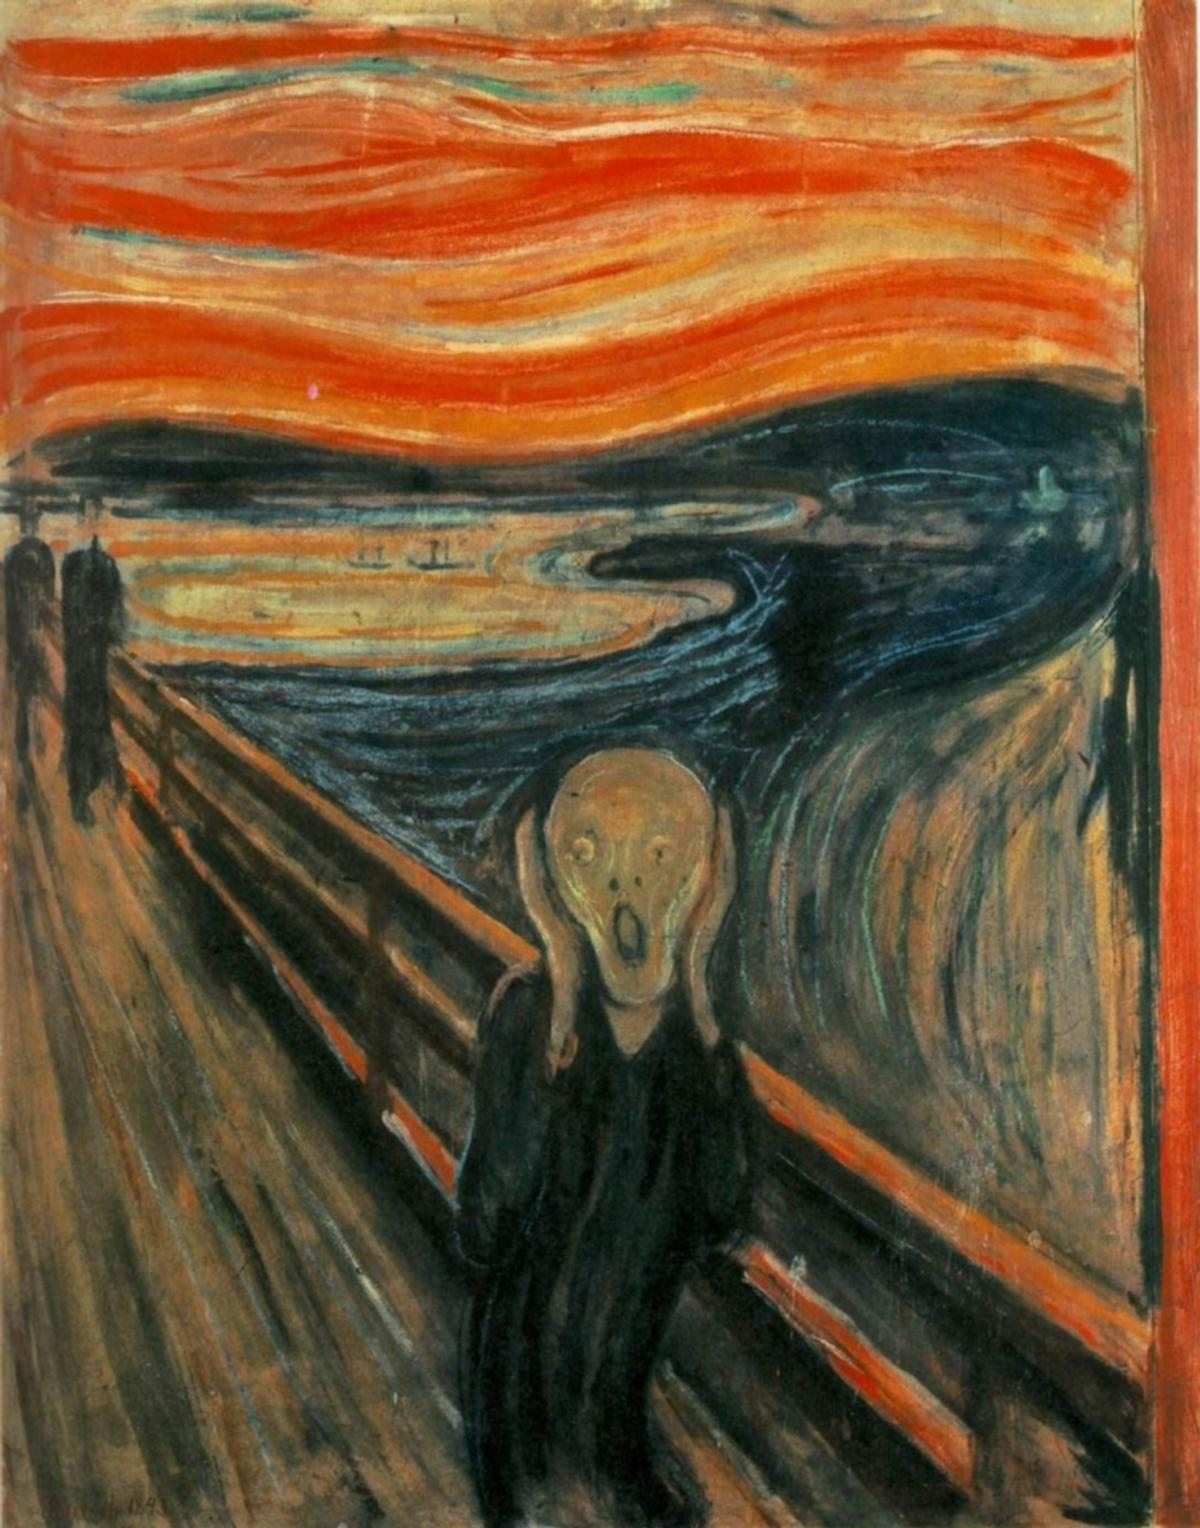
\includegraphics[height=0.2\textheight]{./img/the_scream.jpg}}
	    & \subfloat[Imagen de Contenido: Fotografia del Golden Gate]{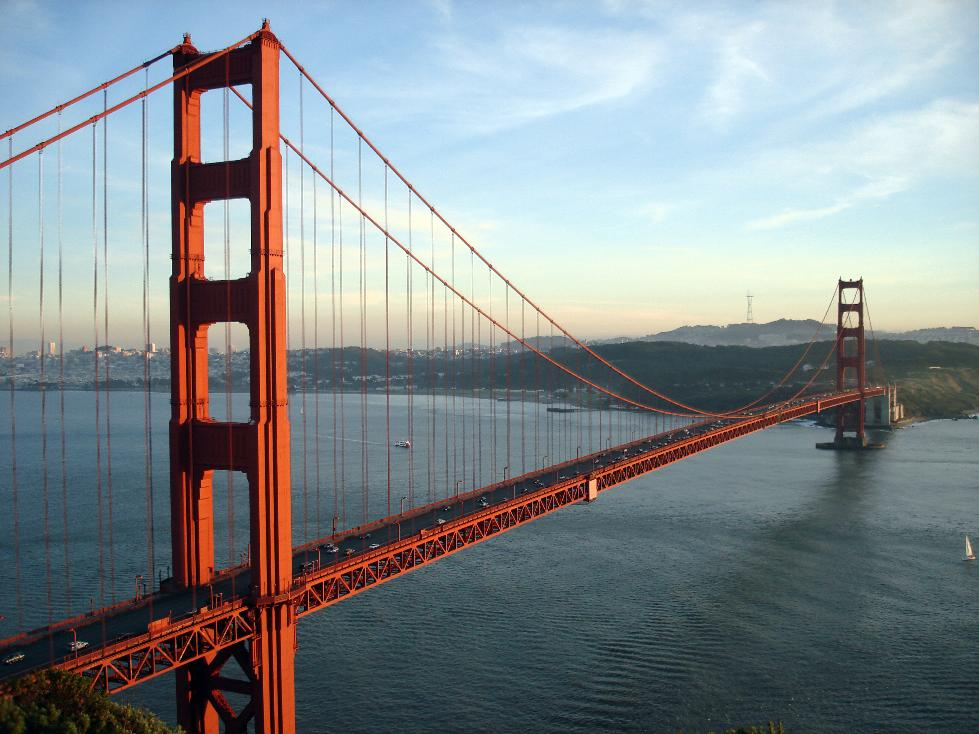
\includegraphics[height=0.2\textheight]{./img/golden_gate.jpg}}\\
	    \subfloat[Resultado comenzando desde ruido]{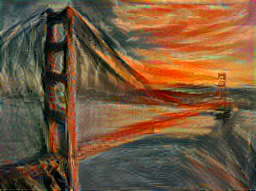
\includegraphics[ height=0.2\textheight]{./img/golden_gate_the_scream_540_random.png}}
	    & \subfloat[Resultado comenzando desde el contenido]{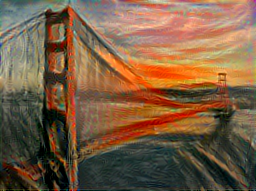
\includegraphics[height=0.2\textheight]{./img/golden_gate_the_scream_540_image.png}}\\
	  \end{tabular}
	  \end{tabularx}
	  \caption{Ejemplos de obras de arte correspondientes a los estilos seleccionados}\label{fig:caso2_scream}
	\end{figure}
      
      Al analizar la evolucion de los puntajes predichos por el clasificador nos encontramos con la sorpresa de que el puntaje maximo de clasificación varia dependiendo de la imagen
      en la cual comienza el proceso de tranferencia de estilo, como se puede ver en la figura \ref {fig:puntajes_caso2}, en el grafico (a) se muestra la evolucion de los puntajes
      partiendo de la imagen de ruido, que luego de las 200 iteraciones se termina normalizando al Expresionismo como predicción, lo cual coincide con la imagen de estilo provista.
      Sin embargo, en el grafico (b) se muestra la evolucion de los puntajes de predicción partiendo de la imagen de contenido, en la cual se exhibe al Simbolismo como prediccion 
      mayoritaria.
      
      \begin{figure}[H]
	\begin{center}
	  \subfloat[Evolucion de los puntajes comenzando desde ruido]{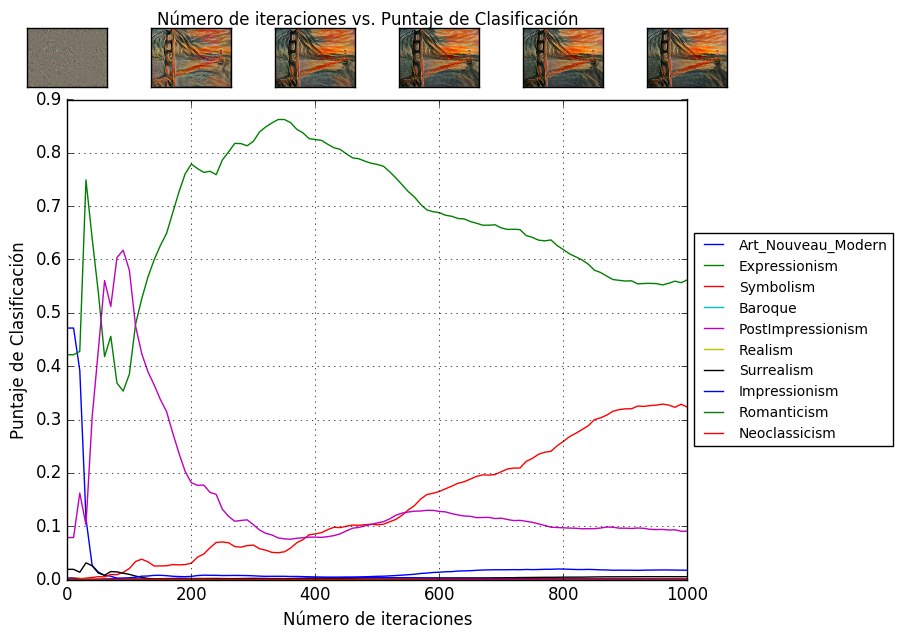
\includegraphics[height=0.4\textheight]{./img/golden_gate_thescream_random_scores.png}}\\
	  \subfloat[Evolucion de los puntajes comenzando desde contenido]{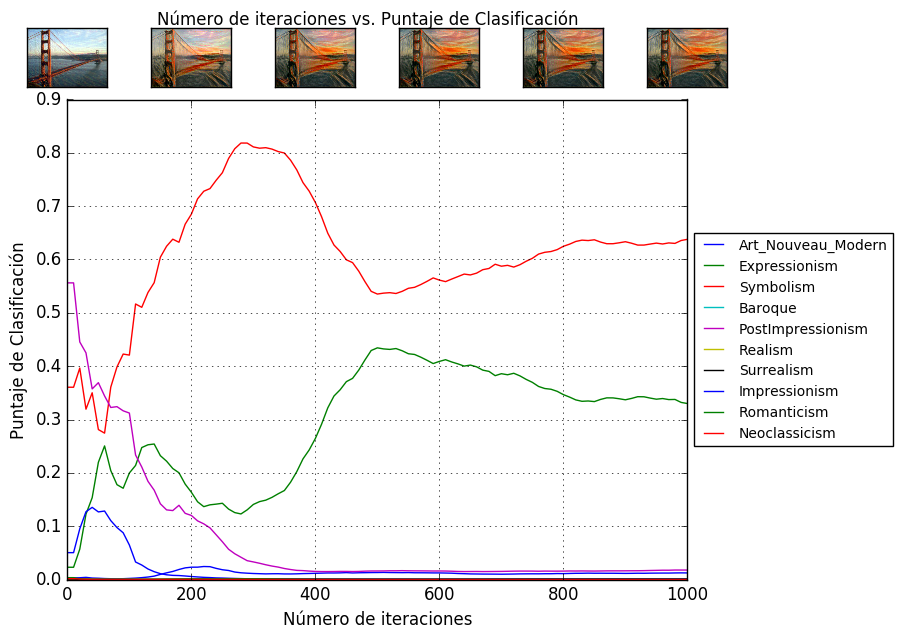
\includegraphics[height=0.4\textheight]{./img/golden_gate_thescream_image_scores.png}}\\
	\end{center}
	\caption{Evolucion de los puntajes}
	\label{fig:puntajes_caso2}
      \end{figure}
      
    \subsection{Validacion de hipotesis para criterio de seleccion}
      Luego se realizar un analisis en varios graficos como los presentados en la seccion anterior se concluyo que la hipotesis sobre que el el puntaje de clasificacion de la imagen
      de estilo y el puntaje de la imagen generada coinciden es falsa, debido a que esto no ocurre en todos los casos analizados, dependiendo de la imagen de contenido el estilo
      que obtiene mayor puntaje de clasificacion puede ser distinto al estilo de la imagen de estilo, ya que la imagen de contenido puede influir en el puntaje de clasificacion de estilo
      de la imagen generada, aunque en mucho menor proporción respecto a la imagen de estilo. Este resultado avala la idea que presenta Gatys acerca de que el estilo y el contenido de una
      imagen no son absolutamente separables.\\
      Debido a esto, el criterio de seleccion que se definio para elegir la imagen optima fue el siguiente: el estilo objetivo, en lugar de ser el estilo correspondiente a la imagen de estilo
      provista para la transferencia de estilo, se definio como el estilo que tiene asignada una mayor
      probabilidad de reconocimiento luego de 1000 iteraciones. Una vez definido el estilo objetivo, se definen los intervalos donde el puntaje obtenido por el estilo objetivo
      supera al puntaje del resto de los estilos. La imagen optima elegida es la correspondiente al numero de iteraciones medio del intervalo donde el estilo objetivo es el maximo. En caso de que haya mas de un de
      un intervalo que cumpla con este requisito, se devuelve una imagen optima de cada intervalo como posibles imagenes optimas para que el usuario elija cual es la optima segun su criterio
      cualitativo.


\chapter{Conclusiones, Perspectivas y trabajos a futuro}
  \section{Conclusiones}
  \section{Trabajos a futuro}
    \FIXME{ \url{https://dailyvisionblog.wordpress.com/2016/07/31/notes-on-texture-networks-feed-forward-synthesis-of-textures-and-stylized-images-and-style-transfer-related-papers/}}
    \subsection{Reconocimiento de Estilos}
      Basandose en la misma idea de entrenar una red convolucional para reconocer solo 10 estilos, se podria extender esto a todos los estilos y utilizando todas las imagenes disponibles
      en WikiArt.
    \subsection{Automatizacion de hiperparámetros}
      Se podría realizar una especie de predefinición del número de iteraciones que requiere cada estilo, ejecutando el algoritmo una gran cantidad de veces y definiendo este valor
      estadisticamente, aunque esto puede llegar a no funciónar correctamente en todos los casos ya que dependiendo de la imagen de contenido, el estilo objetivo podria variar.
    \subsection{Compresion de CNN}
      A partir del articulo presentado por Gatys, se fueron publicando una serie de articulos que presentaban mejoras u optimizaciones al algortimo, ademas de buscar comprimir la red,
      para que una vez entrenada en un dispositivo de gran capacidad de computo, luego pueda ser insertado y ejecutado para transferir estilo en dispositivo menor como lo son los smartphones.
      Por ejemplo se lograron entrenar modelos que transfieran el estilo de una obra de arte en particular, que puede ser ejecutado en un smartphone
      
\printindex
\bibliography{./tex/biblio}        %use a bibtex bibliography file refs.bib
\bibliographystyle{unsrt}
\end{document}
